\chapter{Matplotlib}

Matplotlib es una biblioteca de trazado de gráficos de bajo nivel en
Python que sirve como una utilidad de visualización.

Matplotlib es de código abierto y fue creado por John D. Hunter.

Está escrito principalmente en Python, algunos segmentos están escritos
en C, Objective-C y Javascript.

\section{Comprobar versión de matplotlib}

Una vez que \texttt{matplotlib} esté instalado es necesario importarlo.
Se puede verificar la versión del paquete con el comando.

\begin{Shaded}
\begin{Highlighting}[]
\ImportTok{import}\NormalTok{ matplotlib}
\BuiltInTok{print}\NormalTok{(matplotlib.\_\_version\_\_)}
\end{Highlighting}
\end{Shaded}

\begin{verbatim}
3.8.3
\end{verbatim}

\section{Pyplot}

La mayoría de las utilidades de \texttt{Matplotlib} se encuentran bajo
el submódulo \texttt{pyplot}, y generalmente se importan bajo el alias
\texttt{plt}:

\begin{Shaded}
\begin{Highlighting}[]
\ImportTok{import}\NormalTok{ matplotlib.pyplot }\ImportTok{as}\NormalTok{ plt}
\end{Highlighting}
\end{Shaded}

Ahora el paquete \texttt{Pyplot} se puede denominar \texttt{plt}.\\

\begin{code} Dibuja una línea en un diagrama desde la posición \((0,0)\) hasta la posición \((6,250)\).

\begin{Shaded}
\begin{Highlighting}[]
\ImportTok{import}\NormalTok{ matplotlib.pyplot }\ImportTok{as}\NormalTok{ plt}
\ImportTok{import}\NormalTok{ numpy }\ImportTok{as}\NormalTok{ np}

\NormalTok{xpoints }\OperatorTok{=}\NormalTok{ np.array([}\DecValTok{0}\NormalTok{, }\DecValTok{6}\NormalTok{])}
\NormalTok{ypoints }\OperatorTok{=}\NormalTok{ np.array([}\DecValTok{0}\NormalTok{, }\DecValTok{250}\NormalTok{])}

\NormalTok{plt.plot(xpoints, ypoints)}
\NormalTok{plt.show()}
\end{Highlighting}
\end{Shaded}
\begin{figure}
  \centering
  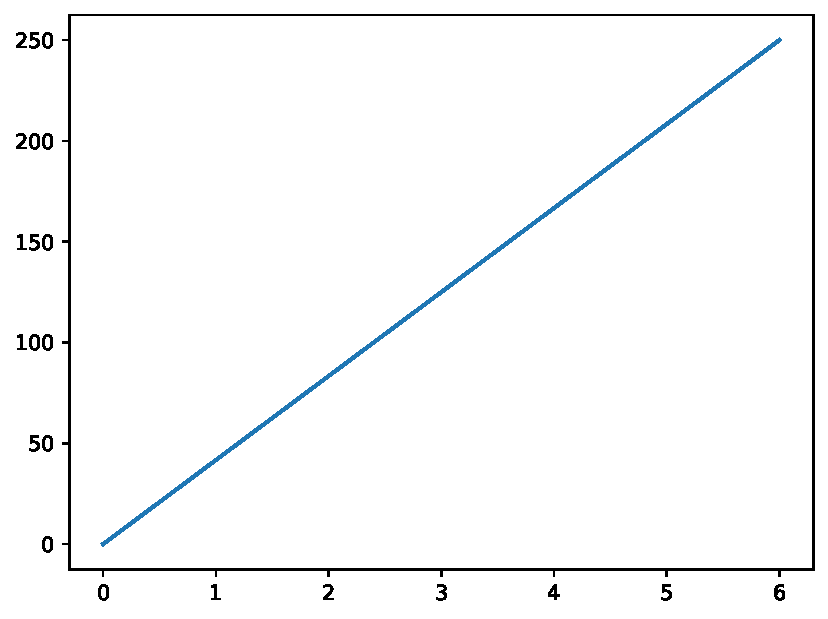
\includegraphics[scale=0.6]{img/grafica1001.pdf}
\end{figure}

\end{code}

\section{Graficas con matplotlib}

\subsection{\texorpdfstring{Gráfica puntos \((x, y)\)}{Gráfica puntos (x, y)}}

La función \texttt{plot()} se utiliza para dibujar puntos en un
diagrama. Por defecto, \texttt{plot()} dibuja una línea de punto a
punto.

La función toma parámetros para especificar puntos en el diagrama.

\begin{itemize}
  \item El parámetro 1 es una matriz que contiene los puntos en el eje X.
  \item El parámetro 2 es una matriz que contiene los puntos en el eje Y.
\end{itemize}

Si necesitamos trazar una línea de (1, 3) a (8, 10), tenemos que pasar
dos matrices {[}1, 8{]} y {[}3, 10{]} a la función de trazado.\\

\begin{code} Dibuje una línea en un diagrama desde la posición (1, 3) a la posición (8, 10)

\begin{Shaded}
\begin{Highlighting}[]
\ImportTok{import}\NormalTok{ matplotlib.pyplot }\ImportTok{as}\NormalTok{ plt}
\ImportTok{import}\NormalTok{ numpy }\ImportTok{as}\NormalTok{ np}

\NormalTok{xpoints }\OperatorTok{=}\NormalTok{ np.array([}\DecValTok{1}\NormalTok{, }\DecValTok{8}\NormalTok{])}
\NormalTok{ypoints }\OperatorTok{=}\NormalTok{ np.array([}\DecValTok{3}\NormalTok{, }\DecValTok{10}\NormalTok{])}

\NormalTok{plt.plot(xpoints, ypoints)}
\NormalTok{plt.show()}
\end{Highlighting}
\end{Shaded}

\begin{figure}
  \centering
  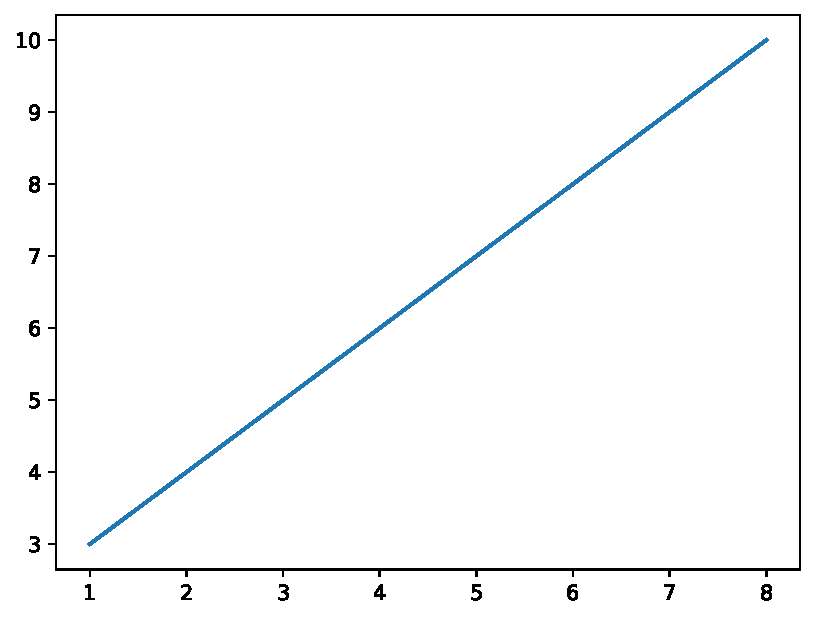
\includegraphics[scale=0.6]{img/grafica1002.pdf}
\end{figure}

\end{code}

\section{Gráfica Sin Línea}

Para trazar solo los marcadores, puede usar notación de cadena de acceso
directo parámetro \texttt{\textquotesingle{}o\textquotesingle{}}, que
significa \emph{\textquotesingle anillos\textquotesingle{}}.\\

\begin{code} Dibuja dos puntos en el diagrama, uno en posición (1, 3) y otro en posición (8, 10).

\begin{Shaded}
\begin{Highlighting}[]
\ImportTok{import}\NormalTok{ matplotlib.pyplot }\ImportTok{as}\NormalTok{ plt}
\ImportTok{import}\NormalTok{ numpy }\ImportTok{as}\NormalTok{ np}

\NormalTok{xpoints }\OperatorTok{=}\NormalTok{ np.array([}\DecValTok{1}\NormalTok{, }\DecValTok{8}\NormalTok{])}
\NormalTok{ypoints }\OperatorTok{=}\NormalTok{ np.array([}\DecValTok{3}\NormalTok{, }\DecValTok{10}\NormalTok{])}

\NormalTok{plt.plot(xpoints, ypoints, }\StringTok{\textquotesingle{}o\textquotesingle{}}\NormalTok{)}
\NormalTok{plt.show()}
\end{Highlighting}
\end{Shaded}

\begin{figure}
  \centering
  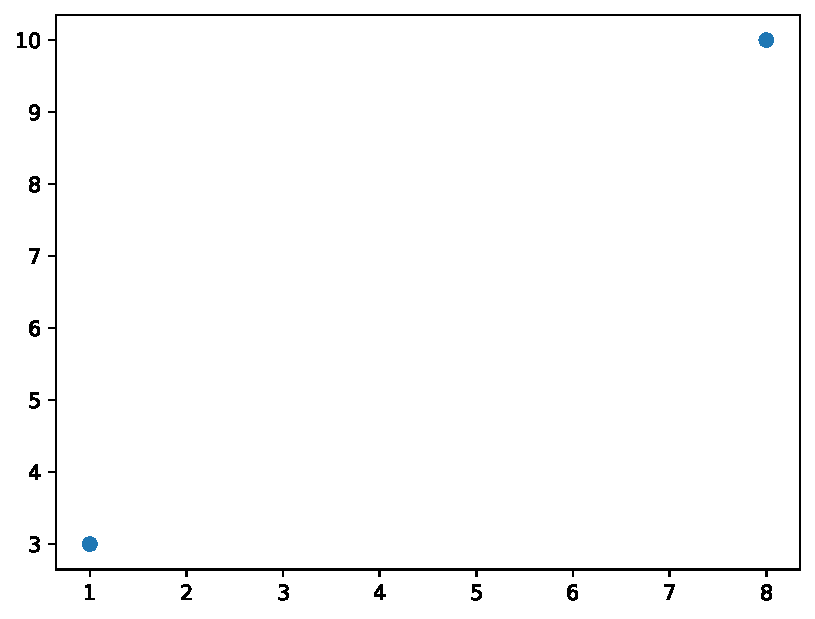
\includegraphics[scale=0.6]{img/grafica1003.pdf}
\end{figure}
\end{code}


\section{Múltiples Puntos}

Puede trazar tantos puntos como desee, solo asegúrese de tener el mismo
número de puntos en ambos ejes. \\

\begin{code} Dibuja una línea en un diagrama desde la posición
\((1, 3)\) a \((2, 8)\) luego a \((6, 1)\) y finalmente a la posición
\((8, 10)\)

\begin{Shaded}
\begin{Highlighting}[]
\ImportTok{import}\NormalTok{ matplotlib.pyplot }\ImportTok{as}\NormalTok{ plt}
\ImportTok{import}\NormalTok{ numpy }\ImportTok{as}\NormalTok{ np}

\NormalTok{xpoints }\OperatorTok{=}\NormalTok{ np.array([}\DecValTok{1}\NormalTok{, }\DecValTok{2}\NormalTok{, }\DecValTok{6}\NormalTok{, }\DecValTok{8}\NormalTok{])}
\NormalTok{ypoints }\OperatorTok{=}\NormalTok{ np.array([}\DecValTok{3}\NormalTok{, }\DecValTok{8}\NormalTok{, }\DecValTok{1}\NormalTok{, }\DecValTok{10}\NormalTok{])}

\NormalTok{plt.plot(xpoints, ypoints)}
\NormalTok{plt.show()}
\end{Highlighting}
\end{Shaded}

\begin{figure}
  \centering
  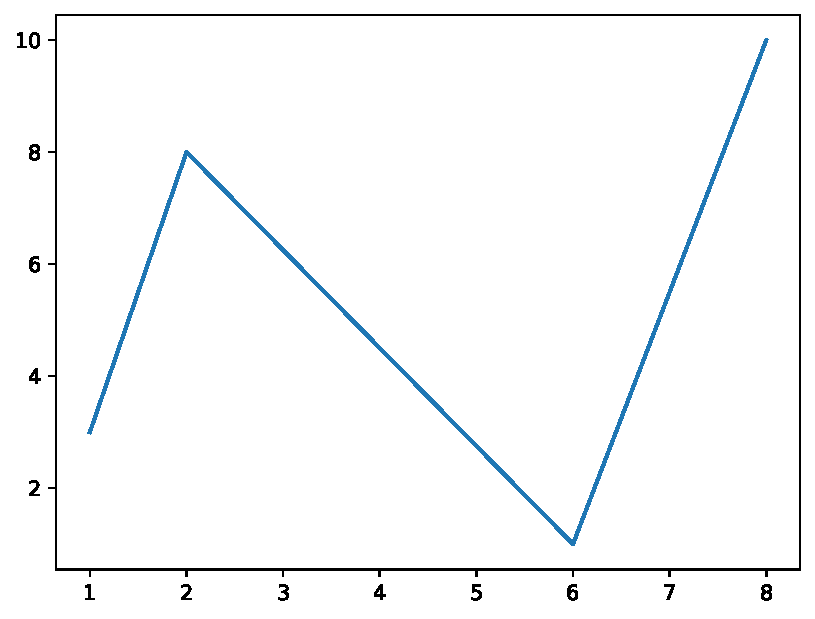
\includegraphics[scale=0.6]{img/grafica1004.pdf}
\end{figure}
\end{code}

\section{\texorpdfstring{Valores \(x\) predeterminados}{Valores x predeterminados}}

Si no especificamos los puntos en el eje \(x\), obtendrán los valores
predeterminados \(0, 1, 2, 3, \dots\), dependiendo de la longitud de los
puntos \(y\).

Entonces, si tomamos el mismo ejemplo que el anterior y dejamos de lado
los puntos \(x\), el diagrama se verá así:\\

\begin{code} Gráfica sin valores \(x\).

\begin{Shaded}
\begin{Highlighting}[]
\ImportTok{import}\NormalTok{ matplotlib.pyplot }\ImportTok{as}\NormalTok{ plt}
\ImportTok{import}\NormalTok{ numpy }\ImportTok{as}\NormalTok{ np}

\NormalTok{ypoints }\OperatorTok{=}\NormalTok{ np.array([}\DecValTok{3}\NormalTok{, }\DecValTok{8}\NormalTok{, }\DecValTok{1}\NormalTok{, }\DecValTok{10}\NormalTok{, }\DecValTok{5}\NormalTok{, }\DecValTok{7}\NormalTok{])}

\NormalTok{plt.plot(ypoints)}
\NormalTok{plt.show()}
\end{Highlighting}
\end{Shaded}

\begin{figure}
  \centering
  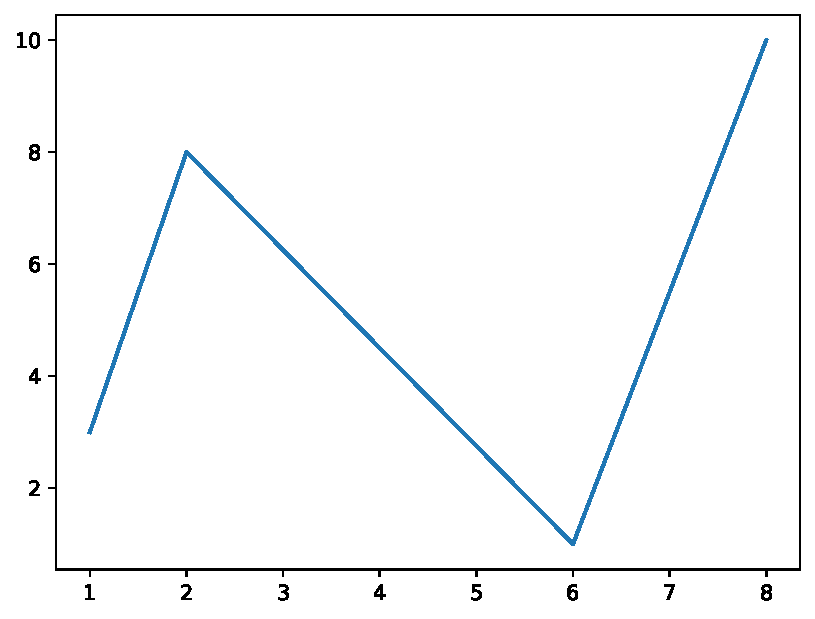
\includegraphics[scale=0.6]{img/grafica1004.pdf}
\end{figure}
\end{code}

\section{Marcadores}

Puede usar el argumento \texttt{marker} para enfatizar cada punto con un
marcador especifico.\\

\begin{code} Marcar cada punto con un círculo.

\begin{Shaded}
\begin{Highlighting}[]
\ImportTok{import}\NormalTok{ matplotlib.pyplot }\ImportTok{as}\NormalTok{ plt}
\ImportTok{import}\NormalTok{ numpy }\ImportTok{as}\NormalTok{ np}

\NormalTok{ypoints }\OperatorTok{=}\NormalTok{ np.array([}\DecValTok{3}\NormalTok{, }\DecValTok{8}\NormalTok{, }\DecValTok{1}\NormalTok{, }\DecValTok{10}\NormalTok{])}

\NormalTok{plt.plot(ypoints, marker }\OperatorTok{=} \StringTok{\textquotesingle{}o\textquotesingle{}}\NormalTok{)}
\NormalTok{plt.show()}
\end{Highlighting}
\end{Shaded}

\begin{figure}
  \centering
  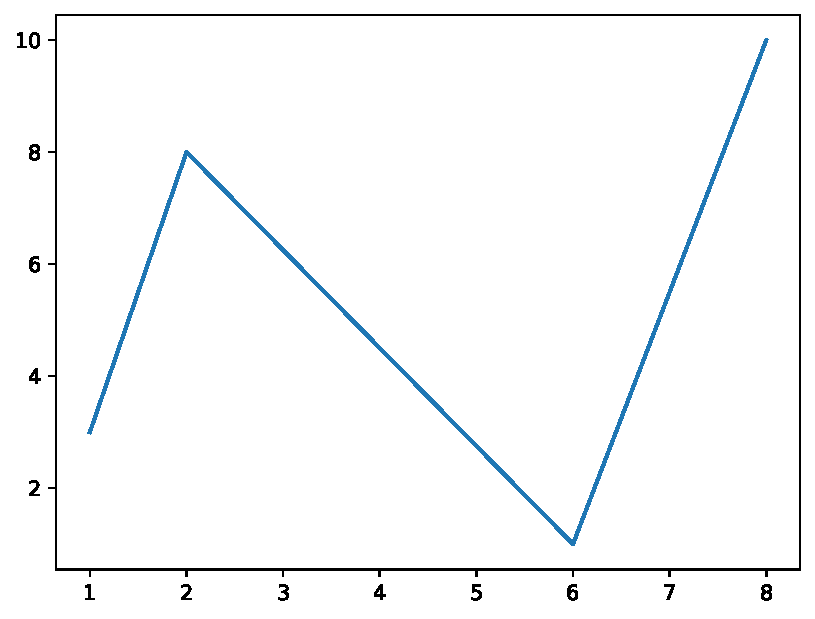
\includegraphics[scale=0.6]{img/grafica1004.pdf}
\end{figure}
\end{code}


\begin{code} Marca cada punto con una estrella.

\begin{Shaded}
\begin{Highlighting}[]
\ImportTok{import}\NormalTok{ matplotlib.pyplot }\ImportTok{as}\NormalTok{ plt}
\ImportTok{import}\NormalTok{ numpy }\ImportTok{as}\NormalTok{ np}

\NormalTok{ypoints }\OperatorTok{=}\NormalTok{ np.array([}\DecValTok{3}\NormalTok{, }\DecValTok{8}\NormalTok{, }\DecValTok{1}\NormalTok{, }\DecValTok{10}\NormalTok{])}

\NormalTok{plt.plot(ypoints, marker }\OperatorTok{=} \StringTok{\textquotesingle{}*\textquotesingle{}}\NormalTok{)}
\NormalTok{plt.show()}
\end{Highlighting}
\end{Shaded}

\begin{figure}
  \centering
  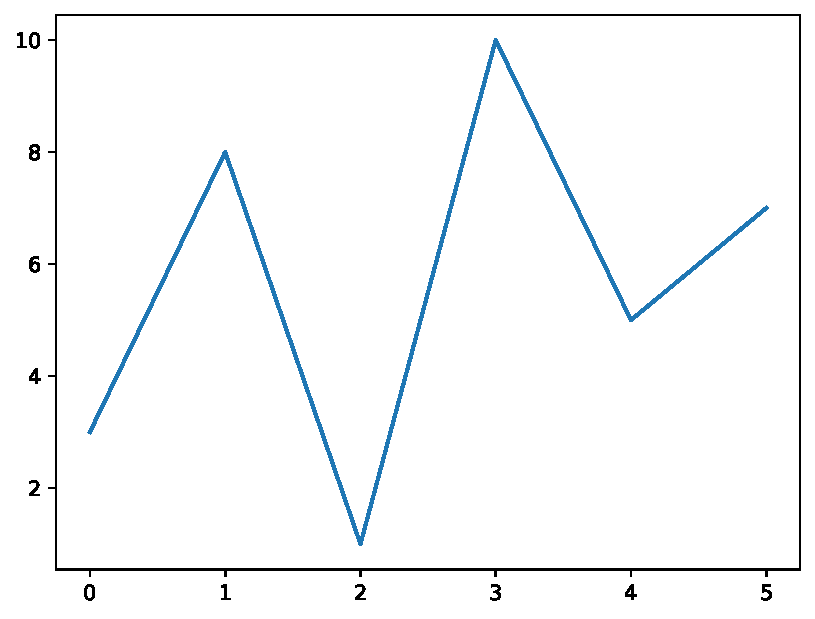
\includegraphics[scale=0.6]{img/grafica1005.pdf}
\end{figure}
\end{code}

\subsection{Referencia de los marcadores}

Puede elegir cualquiera de estos marcadores:

\begin{longtable}[]{@{}cc@{}}
\toprule\noalign{}
Marker & Description \\
\midrule\noalign{}
\endhead
\bottomrule\noalign{}
\endlastfoot
\textquotesingle o\textquotesingle{} & Circle \\
\textquotesingle*\textquotesingle{} & Star \\
\textquotesingle.\textquotesingle{} & Point \\
\textquotesingle,\textquotesingle{} & Pixel \\
\textquotesingle x\textquotesingle{} & X \\
\textquotesingle X\textquotesingle{} & X (filled) \\
\textquotesingle+\textquotesingle{} & Plus \\
\textquotesingle P\textquotesingle{} & Plus (filled) \\
\textquotesingle s\textquotesingle{} & Square \\
\textquotesingle D\textquotesingle{} & Diamond \\
\textquotesingle d\textquotesingle{} & Diamond (thin) \\
\textquotesingle p\textquotesingle{} & Pentagon \\
\textquotesingle H\textquotesingle{} & Hexagon \\
\textquotesingle h\textquotesingle{} & Hexagon \\
\textquotesingle v\textquotesingle{} & Triangle Down \\
\textquotesingle\^{}\textquotesingle{} & Triangle Up \\
\textquotesingle\textless\textquotesingle{} & Triangle Left \\
\textquotesingle\textgreater\textquotesingle{} & Triangle Right \\
\textquotesingle1\textquotesingle{} & Tri Down \\
\textquotesingle2\textquotesingle{} & Tri Up \\
\textquotesingle3\textquotesingle{} & Tri Left \\
\textquotesingle4\textquotesingle{} & Tri Right \\
\textquotesingle{} & \textquotesingle{} \\
\textquotesingle\_\textquotesingle{} & Hline \\
\end{longtable}

\begin{code} Marcador cuadrado.
\begin{Shaded}
\begin{Highlighting}[]
\NormalTok{plt.plot(ypoints, marker }\OperatorTok{=} \StringTok{\textquotesingle{}s\textquotesingle{}}\NormalTok{)}
\NormalTok{plt.show()}
\end{Highlighting}
\end{Shaded}

\begin{figure}
  \centering
  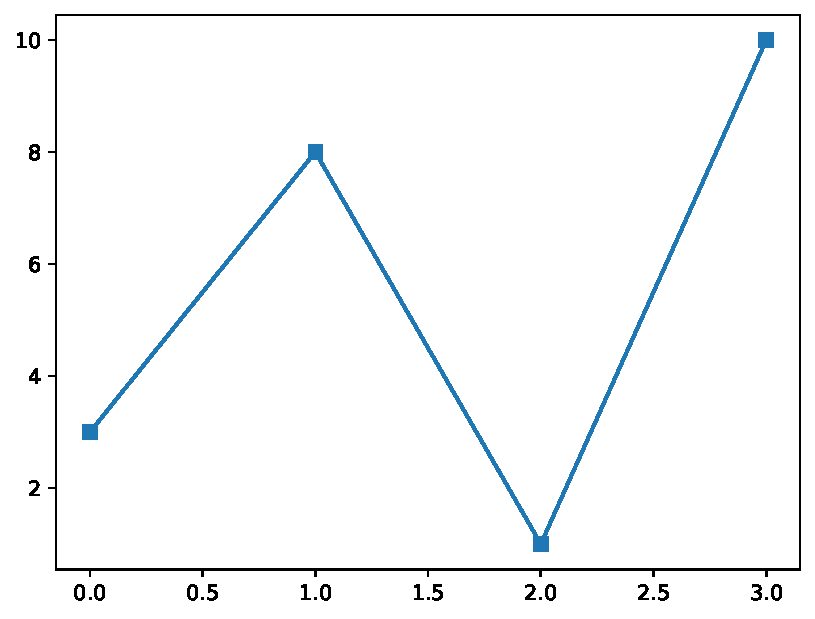
\includegraphics[scale=0.6]{img/grafica1008.pdf}
\end{figure}
\end{code}

\section{\texorpdfstring{Formato cadena \texttt{fmt}}{Formato cadena fmt}}

También puedes usar el notación de cadena de acceso directo parámetro
para especificar el marcador.

Este parámetro también se llama \texttt{fmt} y está escrito con esta
sintaxis:

\begin{Shaded}
\begin{Highlighting}[]
\NormalTok{marker}\OperatorTok{|}\NormalTok{line}\OperatorTok{|}\NormalTok{color}

\end{Highlighting}
\end{Shaded}

\begin{code} Marque cada punto con un círculo.

\begin{Shaded}
\begin{Highlighting}[]
\ImportTok{import}\NormalTok{ matplotlib.pyplot }\ImportTok{as}\NormalTok{ plt}
\ImportTok{import}\NormalTok{ numpy }\ImportTok{as}\NormalTok{ np}

\NormalTok{ypoints }\OperatorTok{=}\NormalTok{ np.array([}\DecValTok{3}\NormalTok{, }\DecValTok{8}\NormalTok{, }\DecValTok{1}\NormalTok{, }\DecValTok{10}\NormalTok{])}

\NormalTok{plt.plot(ypoints, }\StringTok{\textquotesingle{}o:g\textquotesingle{}}\NormalTok{)}
\NormalTok{plt.show()}
\end{Highlighting}
\end{Shaded}

\begin{figure}
  \centering
  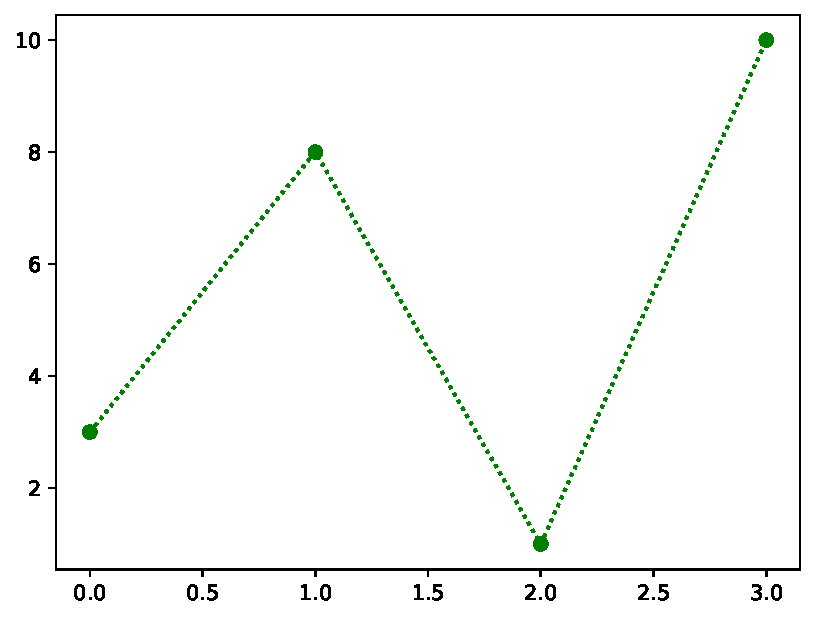
\includegraphics[scale=0.6]{img/grafica1009.pdf}
\end{figure}

\end{code}

El valor del marcador puede ser cualquier cosa de la Referencia del
Marcador anterior.

El valor de la línea puede ser uno de los siguientes:

\subsection{Referencia de Línea}

\begin{longtable}[]{@{}cc@{}}
\toprule\noalign{}
Sintaxis línea & Descripción \\
\midrule\noalign{}
\endhead
\bottomrule\noalign{}
\endlastfoot
\textquotesingle-\textquotesingle{} & Solid line \\
\textquotesingle:\textquotesingle{} & Dotted line 1 \\
\end{longtable}

\textquotesingle-\/-\textquotesingle{} Dashed line
\textquotesingle-.\textquotesingle{} Dashed/dotted line

\begin{Shaded}
\begin{Highlighting}[]
\NormalTok{plt.plot(ypoints, }\StringTok{\textquotesingle{}o{-}.g\textquotesingle{}}\NormalTok{)}
\NormalTok{plt.show()}
\end{Highlighting}
\end{Shaded}

\begin{figure}
  \centering
  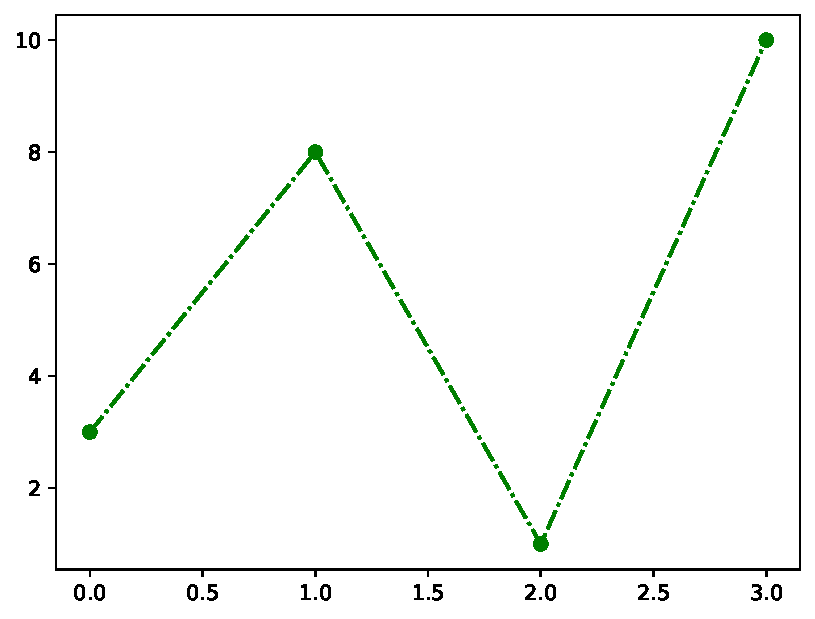
\includegraphics[scale=0.6]{img/grafica1010.pdf}
\end{figure}


\subsection{Referencia de Color}

\begin{longtable}[]{@{}cc@{}}
\toprule\noalign{}
Sintaxis & Descripción \\
\midrule\noalign{}
\endhead
\bottomrule\noalign{}
\endlastfoot
\textquotesingle r\textquotesingle{} & Red \\
\textquotesingle g\textquotesingle{} & Green \\
\textquotesingle b\textquotesingle{} & Blue \\
\textquotesingle c\textquotesingle{} & Cyan \\
\textquotesingle m\textquotesingle{} & Magenta \\
\textquotesingle y\textquotesingle{} & Yellow \\
\textquotesingle k\textquotesingle{} & Black \\
\textquotesingle w\textquotesingle{} & White \\
\end{longtable}

\subsection{Tamaño del Marcador}

Puede usar el argumento de palabra clave \texttt{markersize} o la
versión más corta, \texttt{ms} para establecer el tamaño de los
marcadores.\\

\begin{code} Establezca el tamaño de los marcadores en 20.

\begin{Shaded}
\begin{Highlighting}[]
\ImportTok{import}\NormalTok{ matplotlib.pyplot }\ImportTok{as}\NormalTok{ plt}
\ImportTok{import}\NormalTok{ numpy }\ImportTok{as}\NormalTok{ np}

\NormalTok{ypoints }\OperatorTok{=}\NormalTok{ np.array([}\DecValTok{3}\NormalTok{, }\DecValTok{8}\NormalTok{, }\DecValTok{1}\NormalTok{, }\DecValTok{10}\NormalTok{])}

\NormalTok{plt.plot(ypoints, marker }\OperatorTok{=} \StringTok{\textquotesingle{}o\textquotesingle{}}\NormalTok{, ms }\OperatorTok{=} \DecValTok{20}\NormalTok{)}
\NormalTok{plt.show()}
\end{Highlighting}
\end{Shaded}

\begin{figure}
  \centering
  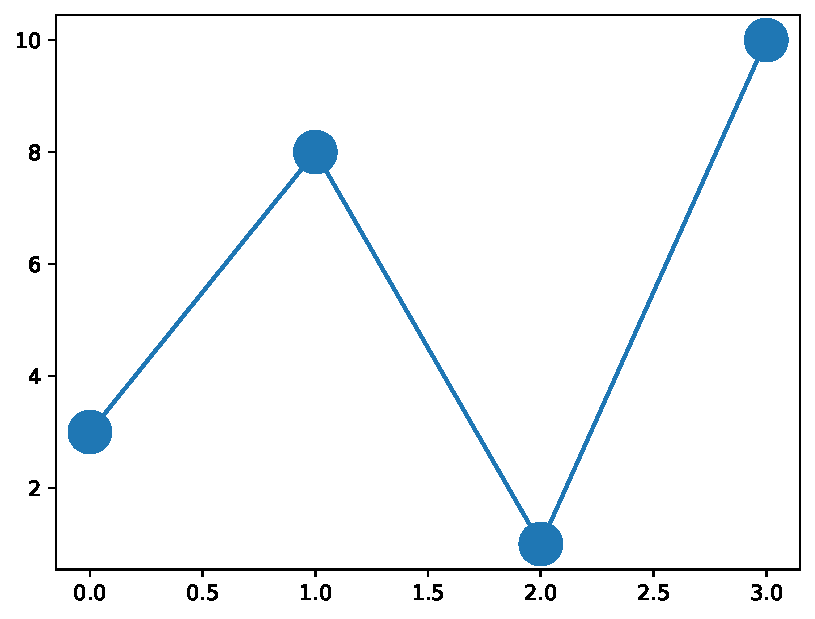
\includegraphics[scale=0.6]{img/grafica1011.pdf}
\end{figure}

\end{code}

\subsection{Color del Marcador}

Puede usar el argumento de palabra clave \texttt{markeredgecolor} o el
más corto \texttt{mec} para establecer el color de la borde de los
marcadores.\\

\begin{code} Establezca el color EDGE en rojo.

\begin{Shaded}
\begin{Highlighting}[]
\ImportTok{import}\NormalTok{ matplotlib.pyplot }\ImportTok{as}\NormalTok{ plt}
\ImportTok{import}\NormalTok{ numpy }\ImportTok{as}\NormalTok{ np}

\NormalTok{ypoints }\OperatorTok{=}\NormalTok{ np.array([}\DecValTok{3}\NormalTok{, }\DecValTok{8}\NormalTok{, }\DecValTok{1}\NormalTok{, }\DecValTok{10}\NormalTok{])}

\NormalTok{plt.plot(ypoints, marker }\OperatorTok{=} \StringTok{\textquotesingle{}o\textquotesingle{}}\NormalTok{, ms }\OperatorTok{=} \DecValTok{20}\NormalTok{, mec }\OperatorTok{=} \StringTok{\textquotesingle{}r\textquotesingle{}}\NormalTok{)}
\NormalTok{plt.show()}
\end{Highlighting}
\end{Shaded}

\begin{figure}
  \centering
  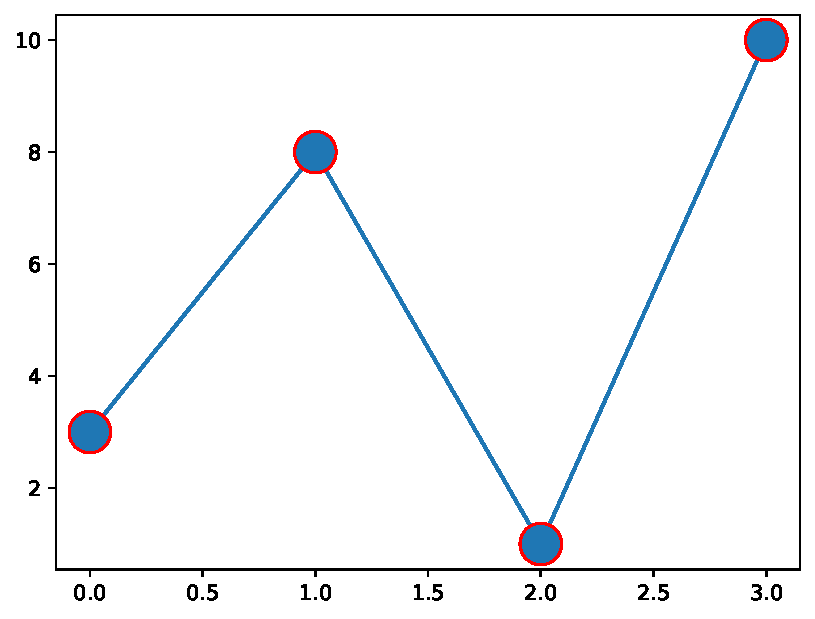
\includegraphics[scale=0.6]{img/grafica1012.pdf}
\end{figure}

\end{code}

Puede usar el argumento de palabra clave \texttt{markerfacecolor} o el
más corto \texttt{mfc} para establecer el color dentro del borde de los
marcadores:\\

\begin{code} Coloque el color FACE en rojo.

\begin{Shaded}
\begin{Highlighting}[]
\ImportTok{import}\NormalTok{ matplotlib.pyplot }\ImportTok{as}\NormalTok{ plt}
\ImportTok{import}\NormalTok{ numpy }\ImportTok{as}\NormalTok{ np}

\NormalTok{ypoints }\OperatorTok{=}\NormalTok{ np.array([}\DecValTok{3}\NormalTok{, }\DecValTok{8}\NormalTok{, }\DecValTok{1}\NormalTok{, }\DecValTok{10}\NormalTok{])}

\NormalTok{plt.plot(ypoints, marker }\OperatorTok{=} \StringTok{\textquotesingle{}o\textquotesingle{}}\NormalTok{, ms }\OperatorTok{=} \DecValTok{20}\NormalTok{, mfc }\OperatorTok{=} \StringTok{\textquotesingle{}r\textquotesingle{}}\NormalTok{)}
\NormalTok{plt.show()}
\end{Highlighting}
\end{Shaded}

\begin{figure}
  \centering
  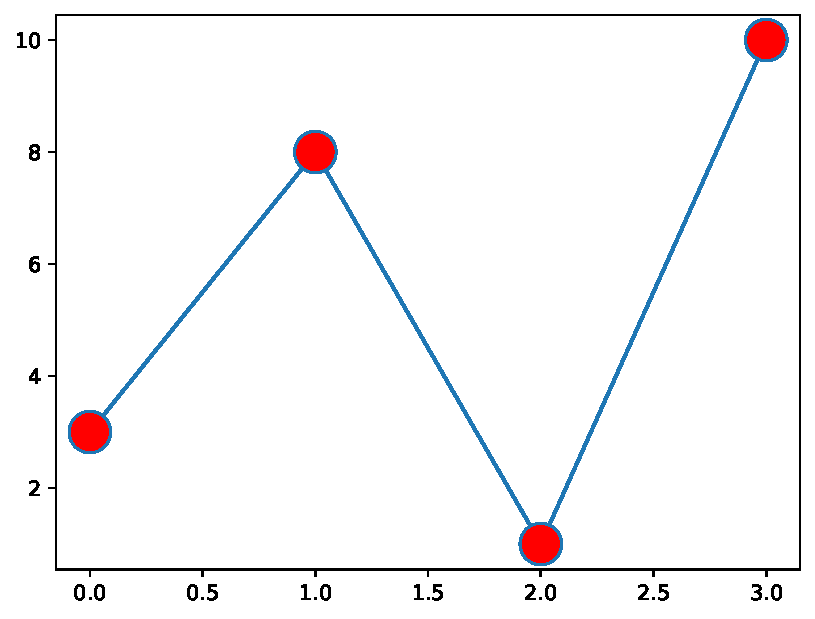
\includegraphics[scale=0.6]{img/grafica1013.pdf}
\end{figure}
\end{code}

Usar ambos el \texttt{mec} y \texttt{mfc} argumentos para colorear todo
el marcador:\\

\begin{code} Establezca el color de ambos borde y el cara a rojo.

\begin{Shaded}
\begin{Highlighting}[]
\ImportTok{import}\NormalTok{ matplotlib.pyplot }\ImportTok{as}\NormalTok{ plt}
\ImportTok{import}\NormalTok{ numpy }\ImportTok{as}\NormalTok{ np}

\NormalTok{ypoints }\OperatorTok{=}\NormalTok{ np.array([}\DecValTok{3}\NormalTok{, }\DecValTok{8}\NormalTok{, }\DecValTok{1}\NormalTok{, }\DecValTok{10}\NormalTok{])}

\NormalTok{plt.plot(ypoints, marker }\OperatorTok{=} \StringTok{\textquotesingle{}o\textquotesingle{}}\NormalTok{, ms }\OperatorTok{=} \DecValTok{20}\NormalTok{, mec }\OperatorTok{=} \StringTok{\textquotesingle{}r\textquotesingle{}}\NormalTok{, mfc }\OperatorTok{=} \StringTok{\textquotesingle{}r\textquotesingle{}}\NormalTok{)}
\NormalTok{plt.show()}
\end{Highlighting}
\end{Shaded}

\begin{figure}
  \centering
  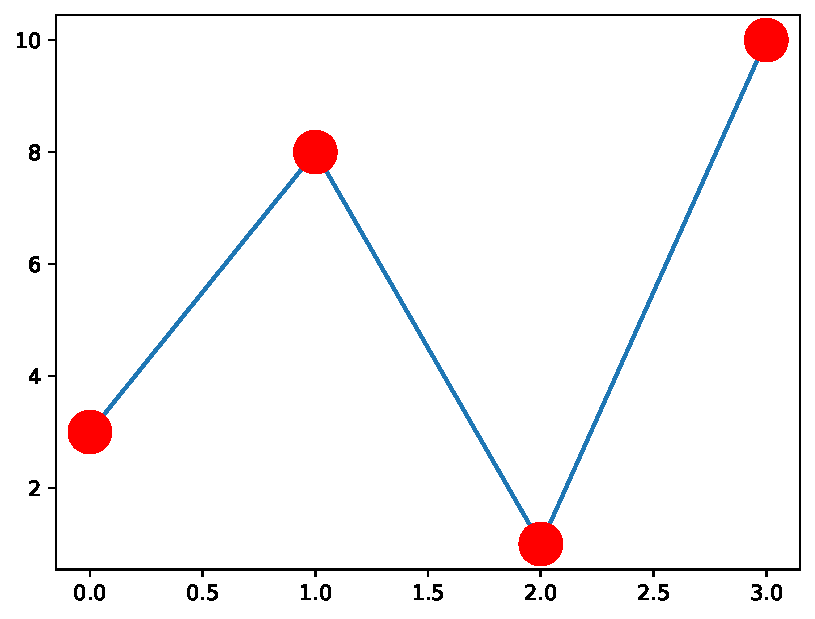
\includegraphics[scale=0.6]{img/grafica1014.pdf}
\end{figure}

\end{code}

También puedes usar valores de color hexadecimal, o cualquiera de los
140 \href{https://www.w3schools.com/colors/colors_names.asp}{nombres de
color} compatibles.

\begin{code} Marque cada punto con un hermoso color verde.

\begin{Shaded}
\begin{Highlighting}[]
\NormalTok{plt.plot(ypoints, marker }\OperatorTok{=} \StringTok{\textquotesingle{}o\textquotesingle{}}\NormalTok{, ms }\OperatorTok{=} \DecValTok{20}\NormalTok{, mec }\OperatorTok{=} \StringTok{\textquotesingle{}\#4CAF50\textquotesingle{}}\NormalTok{, mfc }\OperatorTok{=} \StringTok{\textquotesingle{}\#4CAF50\textquotesingle{}}\NormalTok{)}
\NormalTok{plt.show()}
\end{Highlighting}
\end{Shaded}

\begin{figure}
  \centering
  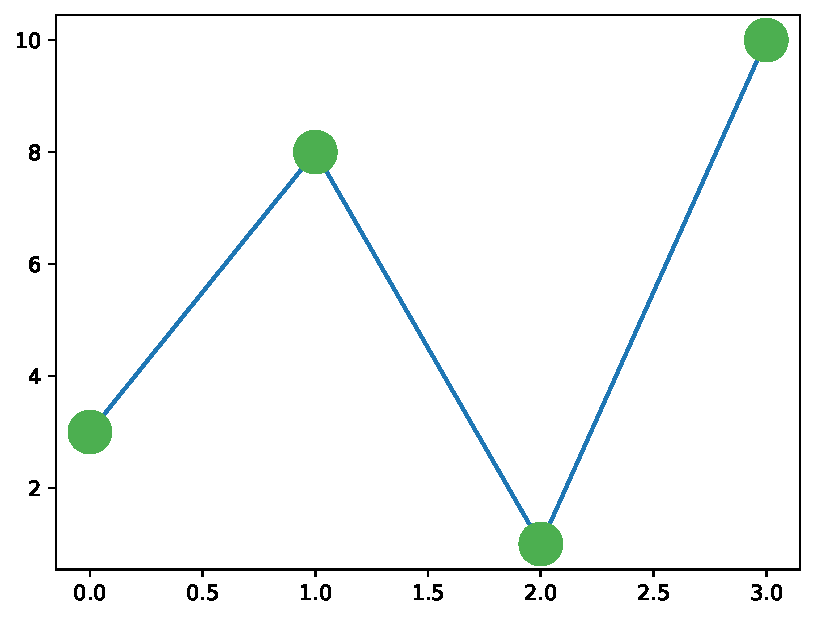
\includegraphics[scale=0.6]{img/grafica1015.pdf}
\end{figure}

\end{code}

\section{Estilo de línea}

Puede usar el argumento de palabra clave \texttt{linestyle}, o más corto
\texttt{ls}, a cambiar el estilo de la línea trazada.\\

\begin{code} Usa una línea punteada.

\begin{Shaded}
\begin{Highlighting}[]
\ImportTok{import}\NormalTok{ matplotlib.pyplot }\ImportTok{as}\NormalTok{ plt}
\ImportTok{import}\NormalTok{ numpy }\ImportTok{as}\NormalTok{ np}

\NormalTok{ypoints }\OperatorTok{=}\NormalTok{ np.array([}\DecValTok{3}\NormalTok{, }\DecValTok{8}\NormalTok{, }\DecValTok{1}\NormalTok{, }\DecValTok{10}\NormalTok{])}

\NormalTok{plt.plot(ypoints, linestyle }\OperatorTok{=} \StringTok{\textquotesingle{}dotted\textquotesingle{}}\NormalTok{)}
\NormalTok{plt.show()}
\end{Highlighting}
\end{Shaded}

\begin{figure}
  \centering
  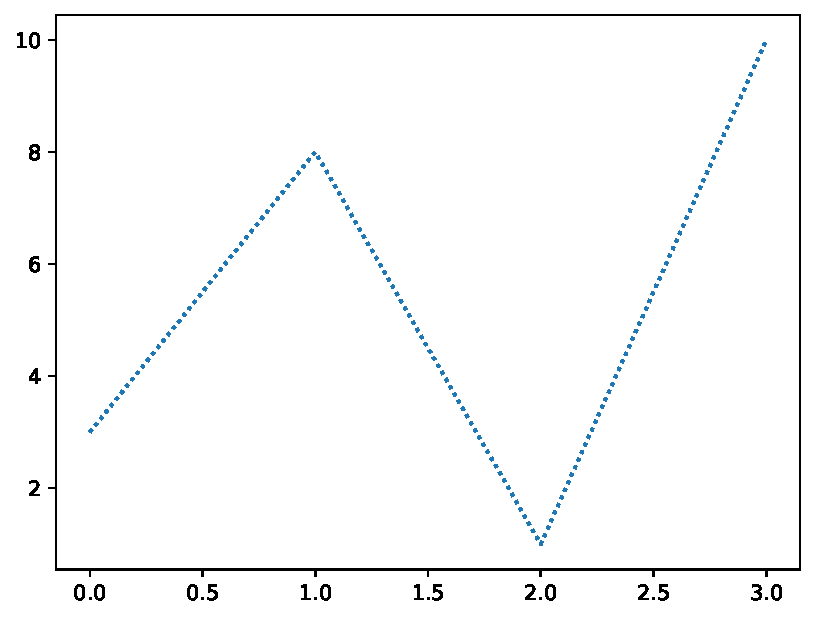
\includegraphics[scale=0.6]{img/grafica1016.pdf}
\end{figure}

\end{code}

\begin{code} Usa una línea discontinua.

\begin{Shaded}
\begin{Highlighting}[]
\NormalTok{plt.plot(ypoints, linestyle }\OperatorTok{=} \StringTok{\textquotesingle{}dashed\textquotesingle{}}\NormalTok{)}
\NormalTok{plt.show()}
\end{Highlighting}
\end{Shaded}

\begin{figure}
  \centering
  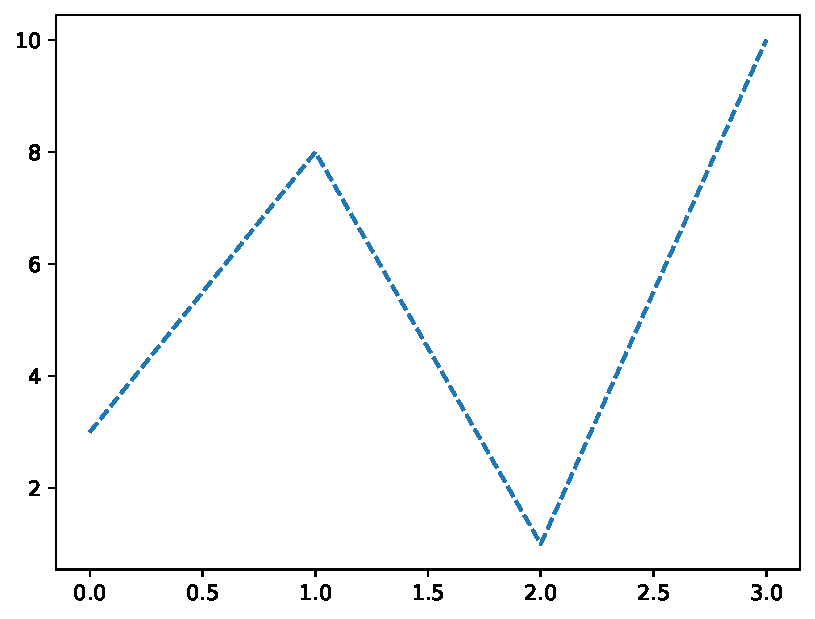
\includegraphics[scale=0.6]{img/grafica1017.pdf}
\end{figure}

\end{code}

\subsection{Sintaxis más corta}

El estilo de línea se puede escribir en una sintaxis más corta:

\begin{itemize}
  \item \texttt{linestyle} se puede escribir como \texttt{ls}.
  \item \texttt{dotted} se puede escribir como \texttt{:}.
  \item \texttt{dashed} se puede escribir como \texttt{-\/-}.
\end{itemize}

\begin{code} Sintaxis más corta.

\begin{Shaded}
\begin{Highlighting}[]
\NormalTok{plt.plot(ypoints, ls }\OperatorTok{=} \StringTok{\textquotesingle{}:\textquotesingle{}}\NormalTok{)}
\NormalTok{plt.show()}
\end{Highlighting}
\end{Shaded}

\begin{figure}
  \centering
  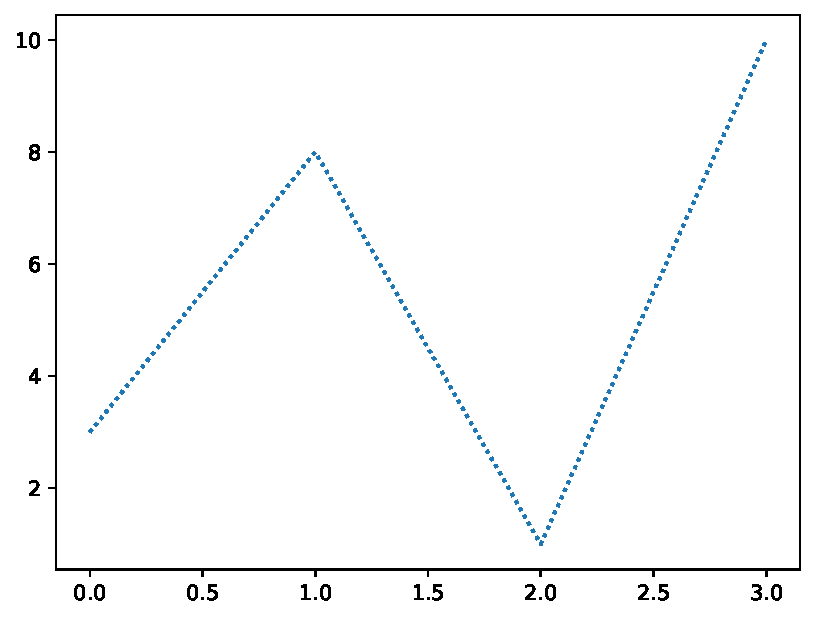
\includegraphics[scale=0.6]{img/grafica1018.pdf}
\end{figure}

\end{code}

\section{Estilos de Línea}

Puedes elegir cualquiera de estos estilos:

\textbar{} Style \textbar{} Or \textbar{}
\textbar:-....:\textbar:-\/-:\textbar{} \textbar{}
\textquotesingle solid\textquotesingle{} \textbar{} (default)
\textquotesingle-\textquotesingle{} \textbar{} \textbar{}
\textquotesingle dotted\textquotesingle{} \textbar{}
\textquotesingle:\textquotesingle{} \textbar{} \textbar{}
\textquotesingle dashed\textquotesingle{} \textbar{}
\textquotesingle-\/-\textquotesingle{} \textbar{} \textbar{}
\textquotesingle dashdot\textquotesingle{} \textbar{}
\textquotesingle-.\textquotesingle{} \textbar{} \textbar{}
\textquotesingle None\textquotesingle{} \textbar{}
\textquotesingle\textquotesingle{} or \textquotesingle{}
\textquotesingle{} \textbar{}

\section{Color de Línea}

Puede usar el argumento de palabra clave \texttt{color} o el más corto
\texttt{c} para establecer el color de la línea.

\begin{code} Establecer el color de la línea en rojo.

\begin{Shaded}
\begin{Highlighting}[]
\ImportTok{import}\NormalTok{ matplotlib.pyplot }\ImportTok{as}\NormalTok{ plt}
\ImportTok{import}\NormalTok{ numpy }\ImportTok{as}\NormalTok{ np}

\NormalTok{ypoints }\OperatorTok{=}\NormalTok{ np.array([}\DecValTok{3}\NormalTok{, }\DecValTok{8}\NormalTok{, }\DecValTok{1}\NormalTok{, }\DecValTok{10}\NormalTok{])}

\NormalTok{plt.plot(ypoints, color }\OperatorTok{=} \StringTok{\textquotesingle{}r\textquotesingle{}}\NormalTok{)}
\NormalTok{plt.show()}
\end{Highlighting}
\end{Shaded}

\begin{figure}
  \centering
  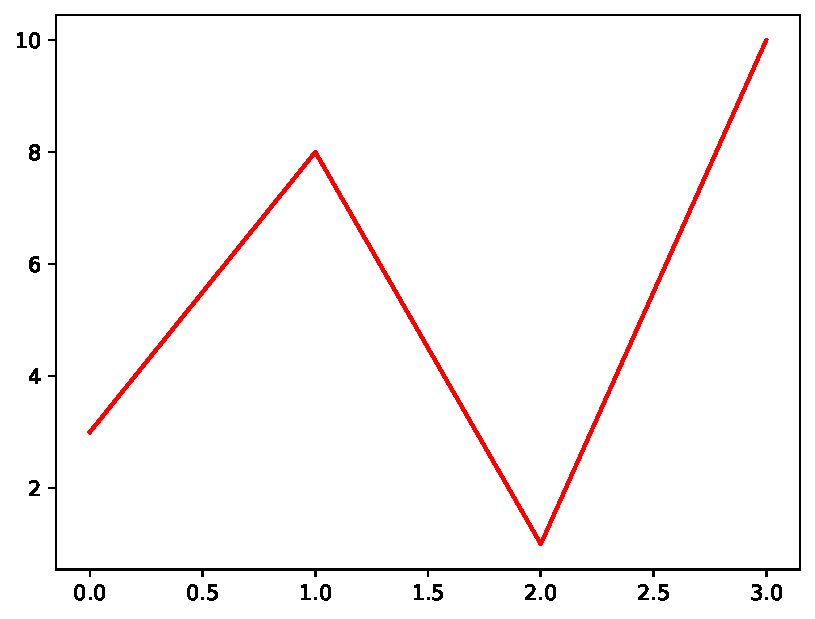
\includegraphics[scale=0.6]{img/grafica1019.pdf}
\end{figure}
\end{code}

También se puede utilizar el color en su valor hexadecimal o los nombres
de color compatibles.

\section{Ancho de Línea}

Puede usar el argumento de palabra clave \texttt{linewidth} o el más
corto \texttt{lw} para cambiar el ancho de la línea.

El valor es un número flotante, en puntos.

\begin{code} Parcela con una línea ancha de 20.5pt.

\begin{Shaded}
\begin{Highlighting}[]
\ImportTok{import}\NormalTok{ matplotlib.pyplot }\ImportTok{as}\NormalTok{ plt}
\ImportTok{import}\NormalTok{ numpy }\ImportTok{as}\NormalTok{ np}

\NormalTok{ypoints }\OperatorTok{=}\NormalTok{ np.array([}\DecValTok{3}\NormalTok{, }\DecValTok{8}\NormalTok{, }\DecValTok{1}\NormalTok{, }\DecValTok{10}\NormalTok{])}

\NormalTok{plt.plot(ypoints, linewidth }\OperatorTok{=} \StringTok{\textquotesingle{}20.5\textquotesingle{}}\NormalTok{)}
\NormalTok{plt.show()}
\end{Highlighting}
\end{Shaded}

\begin{figure}
  \centering
  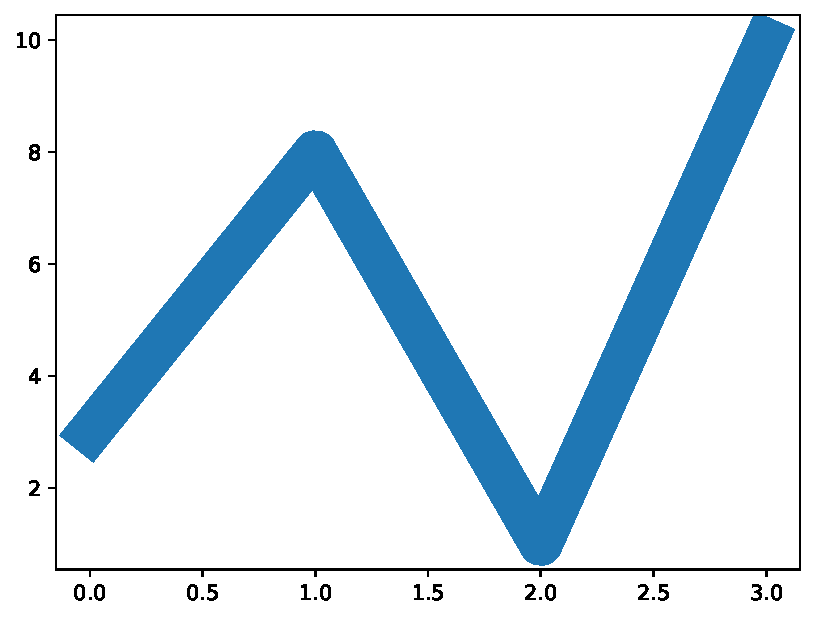
\includegraphics[scale=0.6]{img/grafica1020.pdf}
\end{figure}
\end{code}


\section{Múltiples Líneas}

Puede trazar tantas líneas como desee simplemente agregando más \texttt{plt.plot()} funciones.\\

\begin{code} Dibuja dos líneas especificando un \texttt{plt.plot()} función para cada línea.

\begin{Shaded}
\begin{Highlighting}[]
\ImportTok{import}\NormalTok{ matplotlib.pyplot }\ImportTok{as}\NormalTok{ plt}
\ImportTok{import}\NormalTok{ numpy }\ImportTok{as}\NormalTok{ np}

\NormalTok{y1 }\OperatorTok{=}\NormalTok{ np.array([}\DecValTok{3}\NormalTok{, }\DecValTok{8}\NormalTok{, }\DecValTok{1}\NormalTok{, }\DecValTok{10}\NormalTok{])}
\NormalTok{y2 }\OperatorTok{=}\NormalTok{ np.array([}\DecValTok{6}\NormalTok{, }\DecValTok{2}\NormalTok{, }\DecValTok{7}\NormalTok{, }\DecValTok{11}\NormalTok{])}

\NormalTok{plt.plot(y1)}
\NormalTok{plt.plot(y2)}

\NormalTok{plt.show()}
\end{Highlighting}
\end{Shaded}

\begin{figure}
  \centering
  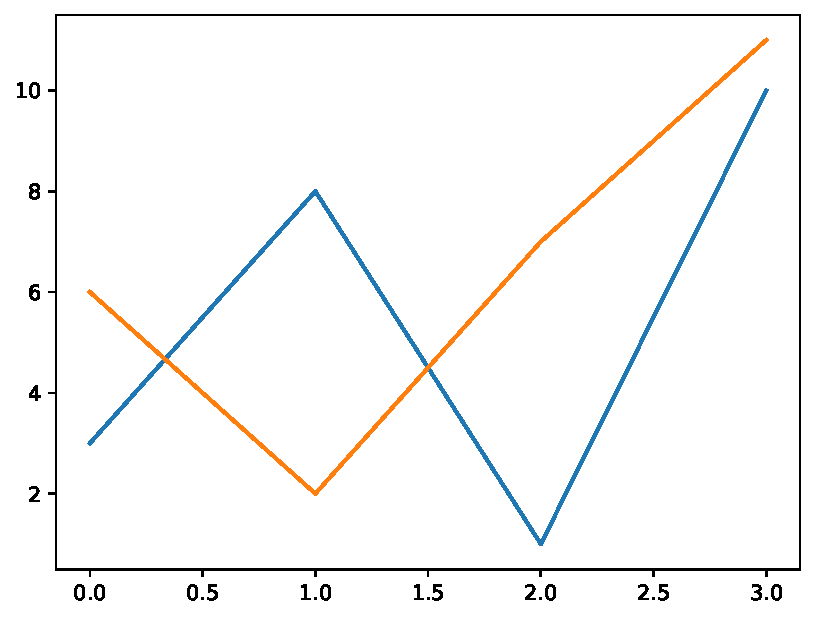
\includegraphics[scale=0.6]{img/grafica1021.pdf}
\end{figure}
\end{code}

También puede trazar muchas líneas agregando los puntos para el eje
\(x\) y \(y\) para cada línea en la misma función \texttt{plt.plot()}.

(En los ejemplos anteriores solo especificamos los puntos en el eje y,
lo que significa que los puntos en el eje x obtuvieron los valores
predeterminados (0, 1, 2, 3).)

Los valores \(x\) y \(y\) vienen en pares.\\

\begin{code} Dibuje dos líneas especificando los valores \(x\) y \(y\) para ambas líneas.

\begin{Shaded}
\begin{Highlighting}[]
\ImportTok{import}\NormalTok{ matplotlib.pyplot }\ImportTok{as}\NormalTok{ plt}
\ImportTok{import}\NormalTok{ numpy }\ImportTok{as}\NormalTok{ np}

\NormalTok{x1 }\OperatorTok{=}\NormalTok{ np.array([}\DecValTok{0}\NormalTok{, }\DecValTok{1}\NormalTok{, }\DecValTok{2}\NormalTok{, }\DecValTok{3}\NormalTok{])}
\NormalTok{y1 }\OperatorTok{=}\NormalTok{ np.array([}\DecValTok{3}\NormalTok{, }\DecValTok{8}\NormalTok{, }\DecValTok{1}\NormalTok{, }\DecValTok{10}\NormalTok{])}
\NormalTok{x2 }\OperatorTok{=}\NormalTok{ np.array([}\DecValTok{0}\NormalTok{, }\DecValTok{1}\NormalTok{, }\DecValTok{2}\NormalTok{, }\DecValTok{3}\NormalTok{])}
\NormalTok{y2 }\OperatorTok{=}\NormalTok{ np.array([}\DecValTok{6}\NormalTok{, }\DecValTok{2}\NormalTok{, }\DecValTok{7}\NormalTok{, }\DecValTok{11}\NormalTok{])}

\NormalTok{plt.plot(x1, y1, x2, y2)}
\NormalTok{plt.show()}
\end{Highlighting}
\end{Shaded}

\begin{figure}
  \centering
  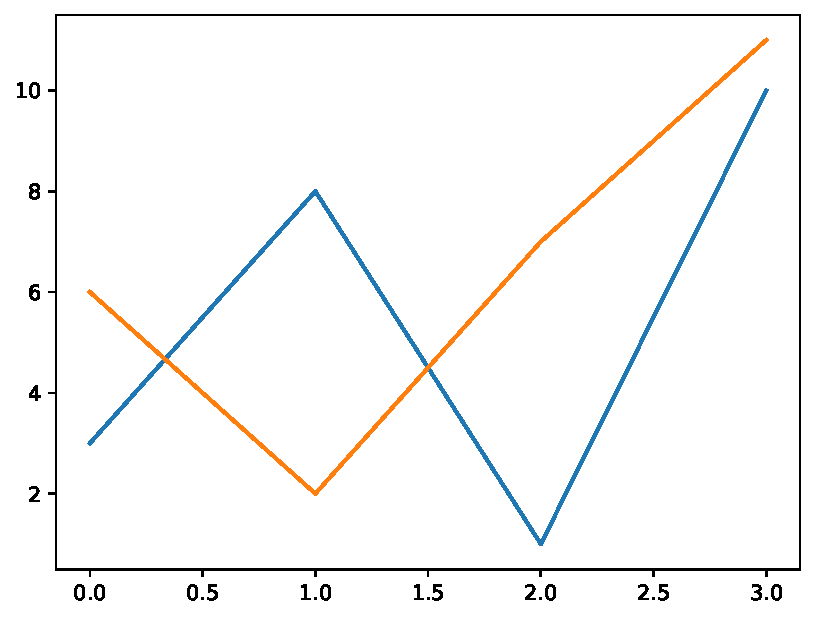
\includegraphics[scale=0.6]{img/grafica1022.pdf}
\end{figure}

\end{code}

\section{Crear Etiquetas para una gráfica}

Con \texttt{Pyplot}, puede usar las funciones \texttt{xlabel()} y
\texttt{ylabel()} para establecer una etiqueta para el eje \(x\) y
\(y\).

\begin{code} Agregar etiquetas al eje \(x\) y \(y\).

\begin{Shaded}
\begin{Highlighting}[]
\ImportTok{import}\NormalTok{ numpy }\ImportTok{as}\NormalTok{ np}
\ImportTok{import}\NormalTok{ matplotlib.pyplot }\ImportTok{as}\NormalTok{ plt}

\NormalTok{x }\OperatorTok{=}\NormalTok{ np.array([}\DecValTok{80}\NormalTok{, }\DecValTok{85}\NormalTok{, }\DecValTok{90}\NormalTok{, }\DecValTok{95}\NormalTok{, }\DecValTok{100}\NormalTok{, }\DecValTok{105}\NormalTok{, }\DecValTok{110}\NormalTok{, }\DecValTok{115}\NormalTok{, }\DecValTok{120}\NormalTok{, }\DecValTok{125}\NormalTok{])}
\NormalTok{y }\OperatorTok{=}\NormalTok{ np.array([}\DecValTok{240}\NormalTok{, }\DecValTok{250}\NormalTok{, }\DecValTok{260}\NormalTok{, }\DecValTok{270}\NormalTok{, }\DecValTok{280}\NormalTok{, }\DecValTok{290}\NormalTok{, }\DecValTok{300}\NormalTok{, }\DecValTok{310}\NormalTok{, }\DecValTok{320}\NormalTok{, }\DecValTok{330}\NormalTok{])}

\NormalTok{plt.plot(x, y)}

\NormalTok{plt.xlabel(}\StringTok{"Average Pulse"}\NormalTok{)}
\NormalTok{plt.ylabel(}\StringTok{"Calorie Burnage"}\NormalTok{)}

\NormalTok{plt.show()}
\end{Highlighting}
\end{Shaded}

\begin{figure}
  \centering
  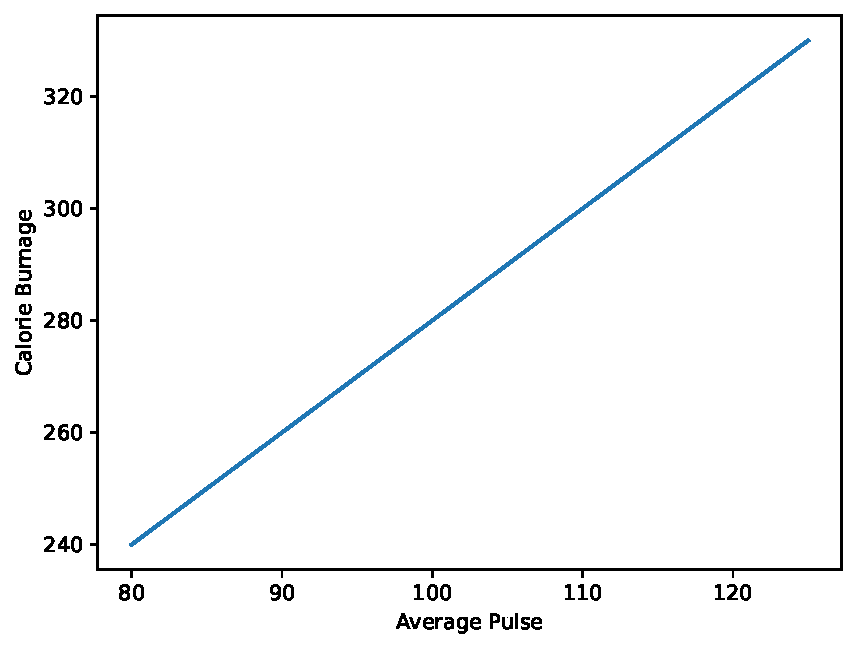
\includegraphics[scale=0.6]{img/grafica1023.pdf}
\end{figure}
\end{code}

\section{Crear un título para una trama}

Con \texttt{Pyplot}, puedes utilizar la función \texttt{title()} para
establecer un título para el gráfico.

\begin{code} Agregue un título de gráfico y etiquetas para los ejes x e y.

\begin{Shaded}
\begin{Highlighting}[]
\ImportTok{import}\NormalTok{ numpy }\ImportTok{as}\NormalTok{ np}
\ImportTok{import}\NormalTok{ matplotlib.pyplot }\ImportTok{as}\NormalTok{ plt}

\NormalTok{x }\OperatorTok{=}\NormalTok{ np.array([}\DecValTok{80}\NormalTok{, }\DecValTok{85}\NormalTok{, }\DecValTok{90}\NormalTok{, }\DecValTok{95}\NormalTok{, }\DecValTok{100}\NormalTok{, }\DecValTok{105}\NormalTok{, }\DecValTok{110}\NormalTok{, }\DecValTok{115}\NormalTok{, }\DecValTok{120}\NormalTok{, }\DecValTok{125}\NormalTok{])}
\NormalTok{y }\OperatorTok{=}\NormalTok{ np.array([}\DecValTok{240}\NormalTok{, }\DecValTok{250}\NormalTok{, }\DecValTok{260}\NormalTok{, }\DecValTok{270}\NormalTok{, }\DecValTok{280}\NormalTok{, }\DecValTok{290}\NormalTok{, }\DecValTok{300}\NormalTok{, }\DecValTok{310}\NormalTok{, }\DecValTok{320}\NormalTok{, }\DecValTok{330}\NormalTok{])}

\NormalTok{plt.plot(x, y)}

\NormalTok{plt.title(}\StringTok{"Sports Watch Data"}\NormalTok{)}
\NormalTok{plt.xlabel(}\StringTok{"Average Pulse"}\NormalTok{)}
\NormalTok{plt.ylabel(}\StringTok{"Calorie Burnage"}\NormalTok{)}

\NormalTok{plt.show()}
\end{Highlighting}
\end{Shaded}

\begin{figure}
  \centering
  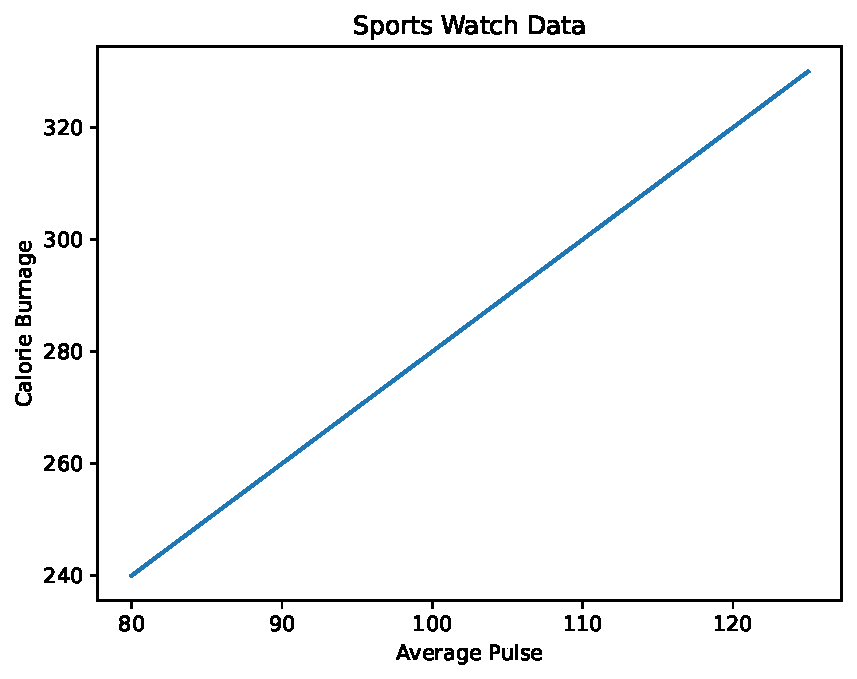
\includegraphics[scale=0.6]{img/grafica1024.pdf}
\end{figure}
\end{code}

\section{Establecer fuente para títulos y etiquetas}

Puede utilizar el parámetro \texttt{fontdict} en \texttt{xlabel()},
\texttt{ylabel()} y \texttt{title()} para establecer las propiedades de
fuente para el título y las etiquetas.

\begin{code} Establecer propiedades de fuente para el título y las etiquetas.

\begin{Shaded}
\begin{Highlighting}[]
\ImportTok{import}\NormalTok{ numpy }\ImportTok{as}\NormalTok{ np}
\ImportTok{import}\NormalTok{ matplotlib.pyplot }\ImportTok{as}\NormalTok{ plt}

\NormalTok{x }\OperatorTok{=}\NormalTok{ np.array([}\DecValTok{80}\NormalTok{, }\DecValTok{85}\NormalTok{, }\DecValTok{90}\NormalTok{, }\DecValTok{95}\NormalTok{, }\DecValTok{100}\NormalTok{, }\DecValTok{105}\NormalTok{, }\DecValTok{110}\NormalTok{, }\DecValTok{115}\NormalTok{, }\DecValTok{120}\NormalTok{, }\DecValTok{125}\NormalTok{])}
\NormalTok{y }\OperatorTok{=}\NormalTok{ np.array([}\DecValTok{240}\NormalTok{, }\DecValTok{250}\NormalTok{, }\DecValTok{260}\NormalTok{, }\DecValTok{270}\NormalTok{, }\DecValTok{280}\NormalTok{, }\DecValTok{290}\NormalTok{, }\DecValTok{300}\NormalTok{, }\DecValTok{310}\NormalTok{, }\DecValTok{320}\NormalTok{, }\DecValTok{330}\NormalTok{])}

\NormalTok{font1 }\OperatorTok{=}\NormalTok{ \{}\StringTok{\textquotesingle{}family\textquotesingle{}}\NormalTok{:}\StringTok{\textquotesingle{}serif\textquotesingle{}}\NormalTok{,}\StringTok{\textquotesingle{}color\textquotesingle{}}\NormalTok{:}\StringTok{\textquotesingle{}blue\textquotesingle{}}\NormalTok{,}\StringTok{\textquotesingle{}size\textquotesingle{}}\NormalTok{:}\DecValTok{20}\NormalTok{\}}
\NormalTok{font2 }\OperatorTok{=}\NormalTok{ \{}\StringTok{\textquotesingle{}family\textquotesingle{}}\NormalTok{:}\StringTok{\textquotesingle{}serif\textquotesingle{}}\NormalTok{,}\StringTok{\textquotesingle{}color\textquotesingle{}}\NormalTok{:}\StringTok{\textquotesingle{}darkred\textquotesingle{}}\NormalTok{,}\StringTok{\textquotesingle{}size\textquotesingle{}}\NormalTok{:}\DecValTok{15}\NormalTok{\}}

\NormalTok{plt.title(}\StringTok{"Sports Watch Data"}\NormalTok{, fontdict }\OperatorTok{=}\NormalTok{ font1)}
\NormalTok{plt.xlabel(}\StringTok{"Average Pulse"}\NormalTok{, fontdict }\OperatorTok{=}\NormalTok{ font2)}
\NormalTok{plt.ylabel(}\StringTok{"Calorie Burnage"}\NormalTok{, fontdict }\OperatorTok{=}\NormalTok{ font2)}

\NormalTok{plt.plot(x, y)}
\NormalTok{plt.show()}
\end{Highlighting}
\end{Shaded}

\begin{figure}
  \centering
  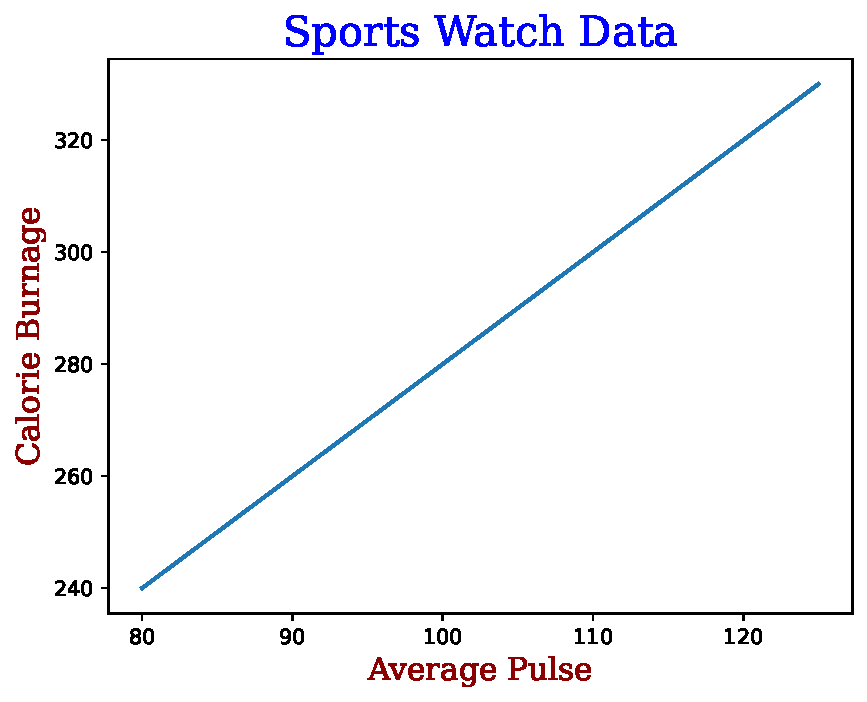
\includegraphics[scale=0.6]{img/grafica1025.pdf}
\end{figure}
\end{code}

\section{Posicionar el título}

Puedes utilizar el parámetro \texttt{loc} en \texttt{title()} para
posicionar el título.

Los valores admitidos son:
\emph{\textquotesingle left\textquotesingle{}},
\emph{\textquotesingle right\textquotesingle{}} y
\emph{\textquotesingle center\textquotesingle{}}. El valor
predeterminado es \emph{\textquotesingle center\textquotesingle{}}.

\begin{code} Coloque el título a la izquierda.

\begin{Shaded}
\begin{Highlighting}[]
\ImportTok{import}\NormalTok{ numpy }\ImportTok{as}\NormalTok{ np}
\ImportTok{import}\NormalTok{ matplotlib.pyplot }\ImportTok{as}\NormalTok{ plt}

\NormalTok{x }\OperatorTok{=}\NormalTok{ np.array([}\DecValTok{80}\NormalTok{, }\DecValTok{85}\NormalTok{, }\DecValTok{90}\NormalTok{, }\DecValTok{95}\NormalTok{, }\DecValTok{100}\NormalTok{, }\DecValTok{105}\NormalTok{, }\DecValTok{110}\NormalTok{, }\DecValTok{115}\NormalTok{, }\DecValTok{120}\NormalTok{, }\DecValTok{125}\NormalTok{])}
\NormalTok{y }\OperatorTok{=}\NormalTok{ np.array([}\DecValTok{240}\NormalTok{, }\DecValTok{250}\NormalTok{, }\DecValTok{260}\NormalTok{, }\DecValTok{270}\NormalTok{, }\DecValTok{280}\NormalTok{, }\DecValTok{290}\NormalTok{, }\DecValTok{300}\NormalTok{, }\DecValTok{310}\NormalTok{, }\DecValTok{320}\NormalTok{, }\DecValTok{330}\NormalTok{])}

\NormalTok{plt.title(}\StringTok{"Sports Watch Data"}\NormalTok{, loc }\OperatorTok{=} \StringTok{\textquotesingle{}left\textquotesingle{}}\NormalTok{)}
\NormalTok{plt.xlabel(}\StringTok{"Average Pulse"}\NormalTok{)}
\NormalTok{plt.ylabel(}\StringTok{"Calorie Burnage"}\NormalTok{)}

\NormalTok{plt.plot(x, y)}
\NormalTok{plt.show()}
\end{Highlighting}
\end{Shaded}

\begin{figure}
  \centering
  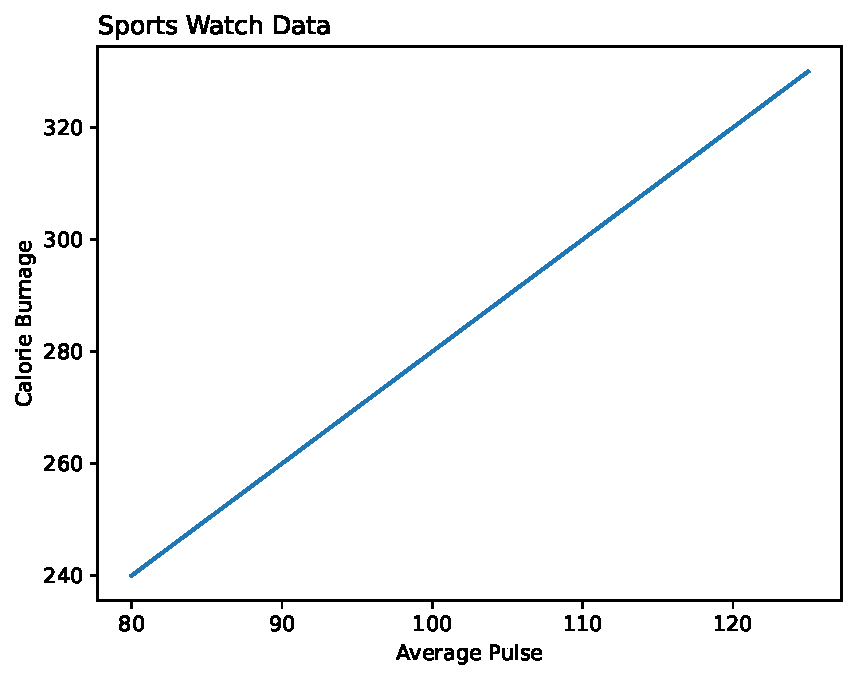
\includegraphics[scale=0.6]{img/grafica1026.pdf}
\end{figure}
\end{code}


\section{Agregar cuadrícula a un gráfico}

Con \texttt{Pyplot}, puedes usar la función \texttt{grid()} para agregar
cuadrícula al gráfico.

\begin{code} Añadir líneas de cuadrícula al gráfico.

\begin{Shaded}
\begin{Highlighting}[]
\ImportTok{import}\NormalTok{ numpy }\ImportTok{as}\NormalTok{ np}
\ImportTok{import}\NormalTok{ matplotlib.pyplot }\ImportTok{as}\NormalTok{ plt}

\NormalTok{x }\OperatorTok{=}\NormalTok{ np.array([}\DecValTok{80}\NormalTok{, }\DecValTok{85}\NormalTok{, }\DecValTok{90}\NormalTok{, }\DecValTok{95}\NormalTok{, }\DecValTok{100}\NormalTok{, }\DecValTok{105}\NormalTok{, }\DecValTok{110}\NormalTok{, }\DecValTok{115}\NormalTok{, }\DecValTok{120}\NormalTok{, }\DecValTok{125}\NormalTok{])}
\NormalTok{y }\OperatorTok{=}\NormalTok{ np.array([}\DecValTok{240}\NormalTok{, }\DecValTok{250}\NormalTok{, }\DecValTok{260}\NormalTok{, }\DecValTok{270}\NormalTok{, }\DecValTok{280}\NormalTok{, }\DecValTok{290}\NormalTok{, }\DecValTok{300}\NormalTok{, }\DecValTok{310}\NormalTok{, }\DecValTok{320}\NormalTok{, }\DecValTok{330}\NormalTok{])}

\NormalTok{plt.title(}\StringTok{"Sports Watch Data"}\NormalTok{)}
\NormalTok{plt.xlabel(}\StringTok{"Average Pulse"}\NormalTok{)}
\NormalTok{plt.ylabel(}\StringTok{"Calorie Burnage"}\NormalTok{)}

\NormalTok{plt.plot(x, y)}
\NormalTok{plt.grid()}
\NormalTok{plt.show()}
\end{Highlighting}
\end{Shaded}

\begin{figure}
  \centering
  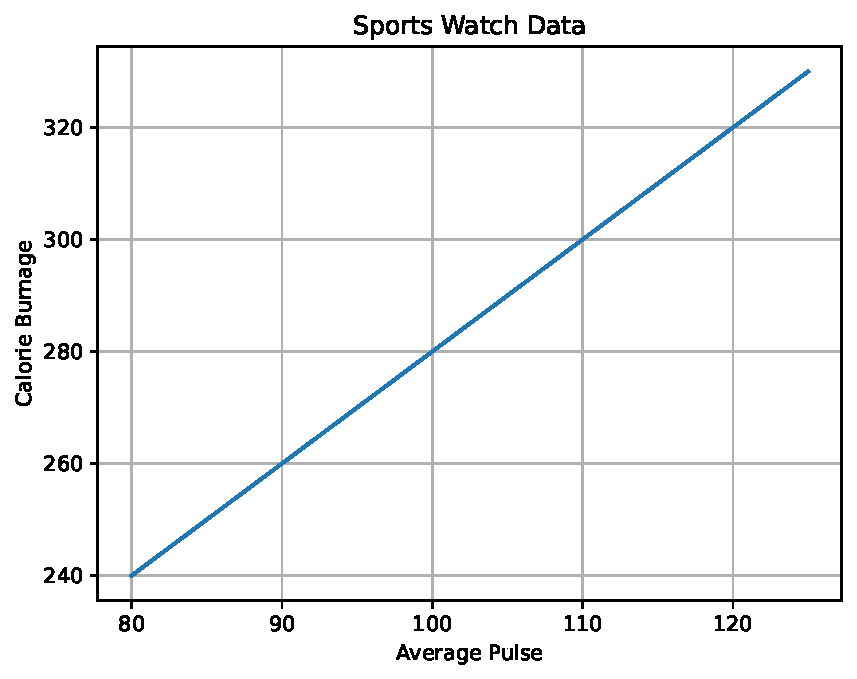
\includegraphics[scale=0.6]{img/grafica1027.pdf}
\end{figure}

\end{code}


\section{Especificar qué líneas de cuadrícula se mostrarán}

Puede utilizar el parámetro \texttt{axis} en la función \texttt{grid()}
para especificar qué líneas de cuadrícula mostrar.

Los valores admitidos son: \emph{\textquotesingle x\textquotesingle{}},
\emph{\textquotesingle y\textquotesingle{}} y
\emph{\textquotesingle both\textquotesingle{}}. El valor predeterminado
es \emph{\textquotesingle both\textquotesingle{}}.

\begin{code} Mostrar solo líneas de cuadrícula para el eje \(x\).

\begin{Shaded}
\begin{Highlighting}[]
\ImportTok{import}\NormalTok{ numpy }\ImportTok{as}\NormalTok{ np}
\ImportTok{import}\NormalTok{ matplotlib.pyplot }\ImportTok{as}\NormalTok{ plt}

\NormalTok{x }\OperatorTok{=}\NormalTok{ np.array([}\DecValTok{80}\NormalTok{, }\DecValTok{85}\NormalTok{, }\DecValTok{90}\NormalTok{, }\DecValTok{95}\NormalTok{, }\DecValTok{100}\NormalTok{, }\DecValTok{105}\NormalTok{, }\DecValTok{110}\NormalTok{, }\DecValTok{115}\NormalTok{, }\DecValTok{120}\NormalTok{, }\DecValTok{125}\NormalTok{])}
\NormalTok{y }\OperatorTok{=}\NormalTok{ np.array([}\DecValTok{240}\NormalTok{, }\DecValTok{250}\NormalTok{, }\DecValTok{260}\NormalTok{, }\DecValTok{270}\NormalTok{, }\DecValTok{280}\NormalTok{, }\DecValTok{290}\NormalTok{, }\DecValTok{300}\NormalTok{, }\DecValTok{310}\NormalTok{, }\DecValTok{320}\NormalTok{, }\DecValTok{330}\NormalTok{])}

\NormalTok{plt.title(}\StringTok{"Sports Watch Data"}\NormalTok{)}
\NormalTok{plt.xlabel(}\StringTok{"Average Pulse"}\NormalTok{)}
\NormalTok{plt.ylabel(}\StringTok{"Calorie Burnage"}\NormalTok{)}

\NormalTok{plt.plot(x, y)}
\NormalTok{plt.grid(axis }\OperatorTok{=} \StringTok{\textquotesingle{}x\textquotesingle{}}\NormalTok{)}
\NormalTok{plt.show()}
\end{Highlighting}
\end{Shaded}

\begin{figure}
  \centering
  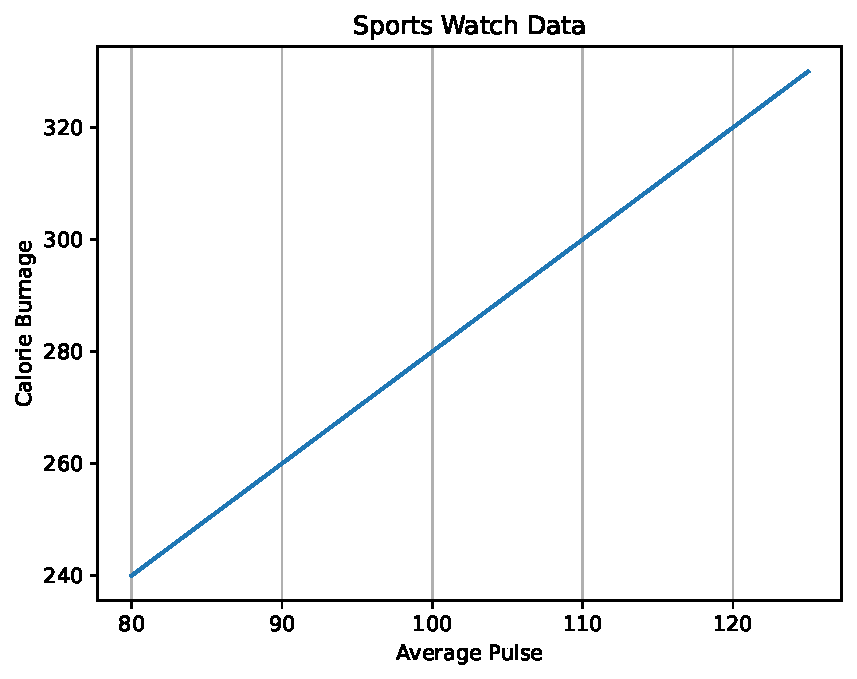
\includegraphics[scale=0.6]{img/grafica1028.pdf}
\end{figure}
\end{code}


\begin{code} Mostrar solo líneas de cuadrícula para el eje \(y\).

\begin{Shaded}
\begin{Highlighting}[]
\ImportTok{import}\NormalTok{ numpy }\ImportTok{as}\NormalTok{ np}
\ImportTok{import}\NormalTok{ matplotlib.pyplot }\ImportTok{as}\NormalTok{ plt}

\NormalTok{x }\OperatorTok{=}\NormalTok{ np.array([}\DecValTok{80}\NormalTok{, }\DecValTok{85}\NormalTok{, }\DecValTok{90}\NormalTok{, }\DecValTok{95}\NormalTok{, }\DecValTok{100}\NormalTok{, }\DecValTok{105}\NormalTok{, }\DecValTok{110}\NormalTok{, }\DecValTok{115}\NormalTok{, }\DecValTok{120}\NormalTok{, }\DecValTok{125}\NormalTok{])}
\NormalTok{y }\OperatorTok{=}\NormalTok{ np.array([}\DecValTok{240}\NormalTok{, }\DecValTok{250}\NormalTok{, }\DecValTok{260}\NormalTok{, }\DecValTok{270}\NormalTok{, }\DecValTok{280}\NormalTok{, }\DecValTok{290}\NormalTok{, }\DecValTok{300}\NormalTok{, }\DecValTok{310}\NormalTok{, }\DecValTok{320}\NormalTok{, }\DecValTok{330}\NormalTok{])}

\NormalTok{plt.title(}\StringTok{"Sports Watch Data"}\NormalTok{)}
\NormalTok{plt.xlabel(}\StringTok{"Average Pulse"}\NormalTok{)}
\NormalTok{plt.ylabel(}\StringTok{"Calorie Burnage"}\NormalTok{)}

\NormalTok{plt.plot(x, y)}
\NormalTok{plt.grid(axis }\OperatorTok{=} \StringTok{\textquotesingle{}y\textquotesingle{}}\NormalTok{)}
\NormalTok{plt.show()}
\end{Highlighting}
\end{Shaded}

\begin{figure}
  \centering
  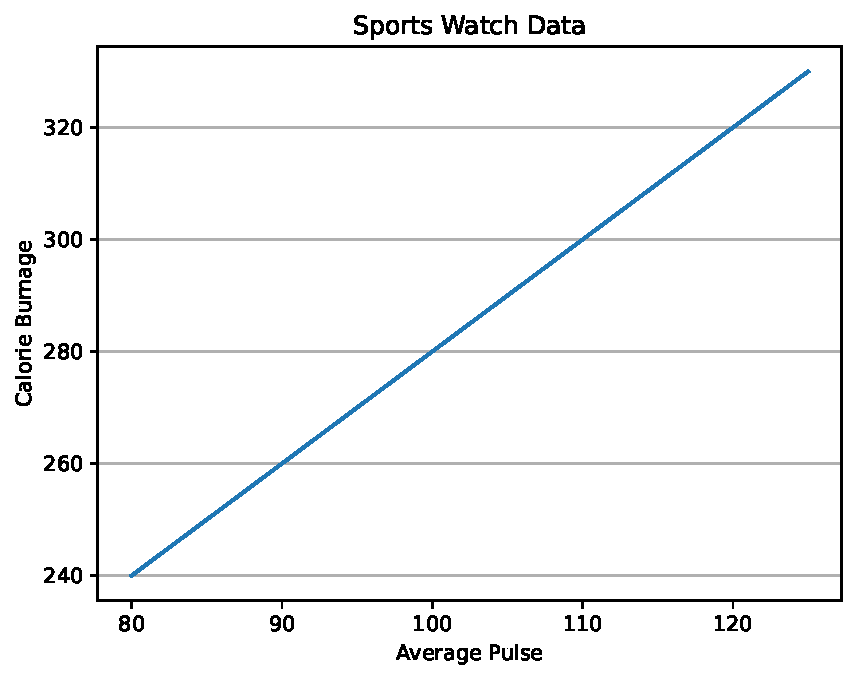
\includegraphics[scale=0.6]{img/grafica1029.pdf}
\end{figure}
\end{code}

\section{Establecer propiedades de línea para la cuadrícula}

También puede configurar las propiedades de línea de la cuadrícula, de esta manera:
\texttt{grid(color\ =\ \textquotesingle{}\_color\_\textquotesingle{},\ linestyle\ =\ \textquotesingle{}\_linestyle\_\textquotesingle{},\ linewidth\ =\ \_number\_)}.

\begin{code} Establecer las propiedades de línea de la cuadrícula.

\begin{Shaded}
\begin{Highlighting}[]
\ImportTok{import}\NormalTok{ numpy }\ImportTok{as}\NormalTok{ np}
\ImportTok{import}\NormalTok{ matplotlib.pyplot }\ImportTok{as}\NormalTok{ plt}

\NormalTok{x }\OperatorTok{=}\NormalTok{ np.array([}\DecValTok{80}\NormalTok{, }\DecValTok{85}\NormalTok{, }\DecValTok{90}\NormalTok{, }\DecValTok{95}\NormalTok{, }\DecValTok{100}\NormalTok{, }\DecValTok{105}\NormalTok{, }\DecValTok{110}\NormalTok{, }\DecValTok{115}\NormalTok{, }\DecValTok{120}\NormalTok{, }\DecValTok{125}\NormalTok{])}
\NormalTok{y }\OperatorTok{=}\NormalTok{ np.array([}\DecValTok{240}\NormalTok{, }\DecValTok{250}\NormalTok{, }\DecValTok{260}\NormalTok{, }\DecValTok{270}\NormalTok{, }\DecValTok{280}\NormalTok{, }\DecValTok{290}\NormalTok{, }\DecValTok{300}\NormalTok{, }\DecValTok{310}\NormalTok{, }\DecValTok{320}\NormalTok{, }\DecValTok{330}\NormalTok{])}

\NormalTok{plt.title(}\StringTok{"Sports Watch Data"}\NormalTok{)}
\NormalTok{plt.xlabel(}\StringTok{"Average Pulse"}\NormalTok{)}
\NormalTok{plt.ylabel(}\StringTok{"Calorie Burnage"}\NormalTok{)}

\NormalTok{plt.plot(x, y)}
\NormalTok{plt.grid(color }\OperatorTok{=} \StringTok{\textquotesingle{}green\textquotesingle{}}\NormalTok{, linestyle }\OperatorTok{=} \StringTok{\textquotesingle{}{-}{-}\textquotesingle{}}\NormalTok{, linewidth }\OperatorTok{=} \FloatTok{0.5}\NormalTok{)}
\NormalTok{plt.show()}
\end{Highlighting}
\end{Shaded}

\begin{figure}
  \centering
  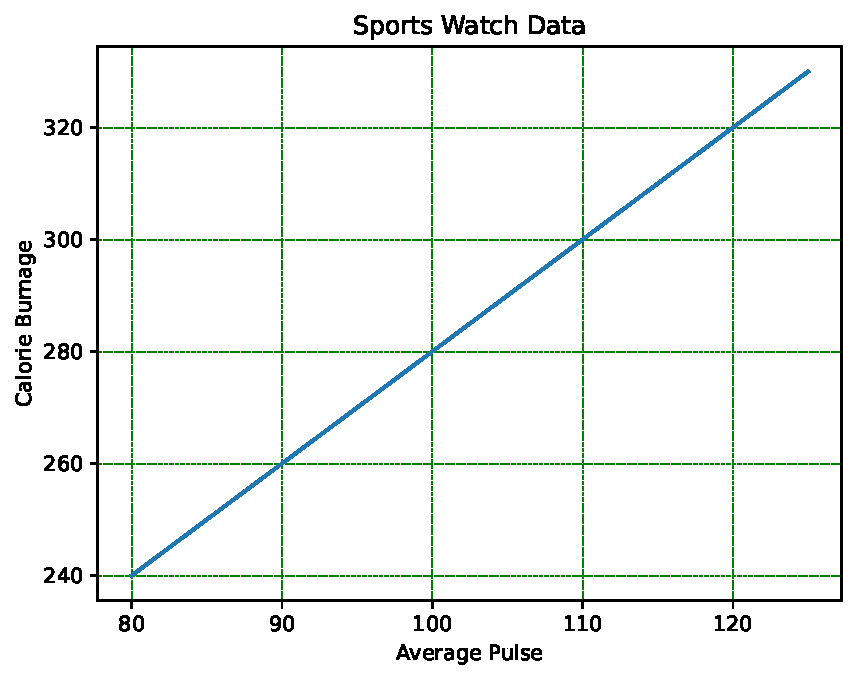
\includegraphics[scale=0.6]{img/grafica1030.pdf}
\end{figure}
\end{code}

\section{Mostrar múltiples gráficos}

Con esta función \texttt{subplot()} puedes dibujar múltiples gráficos en
una figura.

\begin{code} Dibuje 2 gráficos.

\begin{Shaded}
\begin{Highlighting}[]
\ImportTok{import}\NormalTok{ matplotlib.pyplot }\ImportTok{as}\NormalTok{ plt}
\ImportTok{import}\NormalTok{ numpy }\ImportTok{as}\NormalTok{ np}

\CommentTok{\#plot 1:}
\NormalTok{x }\OperatorTok{=}\NormalTok{ np.array([}\DecValTok{0}\NormalTok{, }\DecValTok{1}\NormalTok{, }\DecValTok{2}\NormalTok{, }\DecValTok{3}\NormalTok{])}
\NormalTok{y }\OperatorTok{=}\NormalTok{ np.array([}\DecValTok{3}\NormalTok{, }\DecValTok{8}\NormalTok{, }\DecValTok{1}\NormalTok{, }\DecValTok{10}\NormalTok{])}

\NormalTok{plt.subplot(}\DecValTok{1}\NormalTok{, }\DecValTok{2}\NormalTok{, }\DecValTok{1}\NormalTok{)}
\NormalTok{plt.plot(x,y)}

\CommentTok{\#plot 2:}
\NormalTok{x }\OperatorTok{=}\NormalTok{ np.array([}\DecValTok{0}\NormalTok{, }\DecValTok{1}\NormalTok{, }\DecValTok{2}\NormalTok{, }\DecValTok{3}\NormalTok{])}
\NormalTok{y }\OperatorTok{=}\NormalTok{ np.array([}\DecValTok{10}\NormalTok{, }\DecValTok{20}\NormalTok{, }\DecValTok{30}\NormalTok{, }\DecValTok{40}\NormalTok{])}

\NormalTok{plt.subplot(}\DecValTok{1}\NormalTok{, }\DecValTok{2}\NormalTok{, }\DecValTok{2}\NormalTok{)}
\NormalTok{plt.plot(x,y)}
\NormalTok{plt.show()}
\end{Highlighting}
\end{Shaded}

\begin{figure}
  \centering
  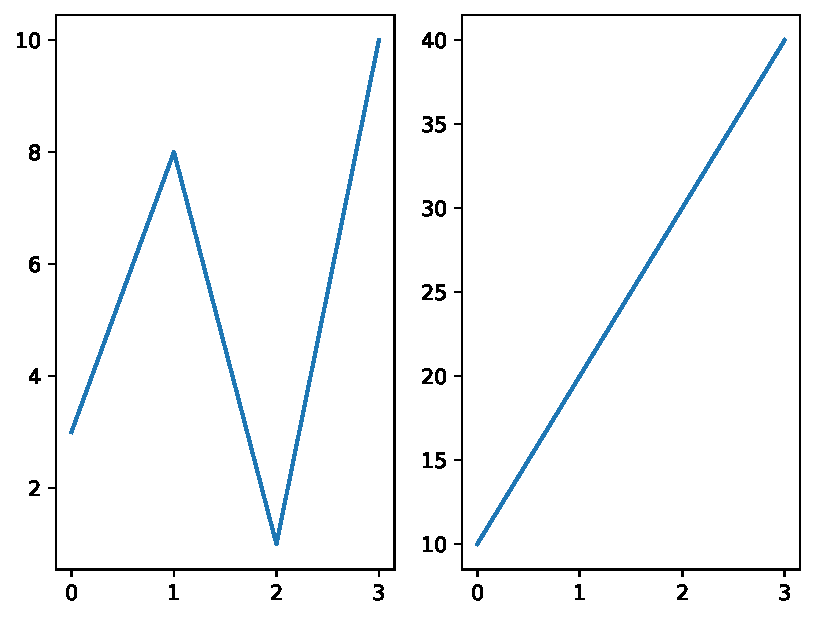
\includegraphics[scale=0.6]{img/grafica1031.pdf}
\end{figure}
\end{code}

\section{La función subplot()}

La función \texttt{subplot()} toma tres argumentos que describen el
diseño de la figura.

El diseño está organizado en filas y columnas, que están representadas
por el primer y segundo argumento.

El tercer argumento representa el índice de la malla actual.

\begin{Shaded}
\begin{Highlighting}[]
\NormalTok{plt.subplot(}\DecValTok{1}\NormalTok{, }\DecValTok{2}\NormalTok{, }\DecValTok{1}\NormalTok{)}
\CommentTok{\#the figure has 1 row, 2 columns, and this plot is the first plot.}
\end{Highlighting}
\end{Shaded}

\begin{Shaded}
\begin{Highlighting}[]
\NormalTok{plt.subplot(}\DecValTok{1}\NormalTok{, }\DecValTok{2}\NormalTok{, }\DecValTok{2}\NormalTok{)}
\CommentTok{\#the figure has 1 row, 2 columns, and this plot is the second plot.}
\end{Highlighting}
\end{Shaded}

Entonces, si queremos una figura con 2 filas y 1 columna (lo que
significa que los dos gráficos se mostrarán uno encima del otro en lugar
de uno al lado del otro), podemos escribir la sintaxis de esta manera.

\begin{code} Dibuje 2 gráficos uno encima del otro.

\begin{Shaded}
\begin{Highlighting}[]
\ImportTok{import}\NormalTok{ matplotlib.pyplot }\ImportTok{as}\NormalTok{ plt}
\ImportTok{import}\NormalTok{ numpy }\ImportTok{as}\NormalTok{ np}

\CommentTok{\#plot 1:}
\NormalTok{x }\OperatorTok{=}\NormalTok{ np.array([}\DecValTok{0}\NormalTok{, }\DecValTok{1}\NormalTok{, }\DecValTok{2}\NormalTok{, }\DecValTok{3}\NormalTok{])}
\NormalTok{y }\OperatorTok{=}\NormalTok{ np.array([}\DecValTok{3}\NormalTok{, }\DecValTok{8}\NormalTok{, }\DecValTok{1}\NormalTok{, }\DecValTok{10}\NormalTok{])}

\NormalTok{plt.subplot(}\DecValTok{2}\NormalTok{, }\DecValTok{1}\NormalTok{, }\DecValTok{1}\NormalTok{)}
\NormalTok{plt.plot(x,y)}

\CommentTok{\#plot 2:}
\NormalTok{x }\OperatorTok{=}\NormalTok{ np.array([}\DecValTok{0}\NormalTok{, }\DecValTok{1}\NormalTok{, }\DecValTok{2}\NormalTok{, }\DecValTok{3}\NormalTok{])}
\NormalTok{y }\OperatorTok{=}\NormalTok{ np.array([}\DecValTok{10}\NormalTok{, }\DecValTok{20}\NormalTok{, }\DecValTok{30}\NormalTok{, }\DecValTok{40}\NormalTok{])}

\NormalTok{plt.subplot(}\DecValTok{2}\NormalTok{, }\DecValTok{1}\NormalTok{, }\DecValTok{2}\NormalTok{)}
\NormalTok{plt.plot(x,y)}
\NormalTok{plt.show()}
\end{Highlighting}
\end{Shaded}

\begin{figure}
  \centering
  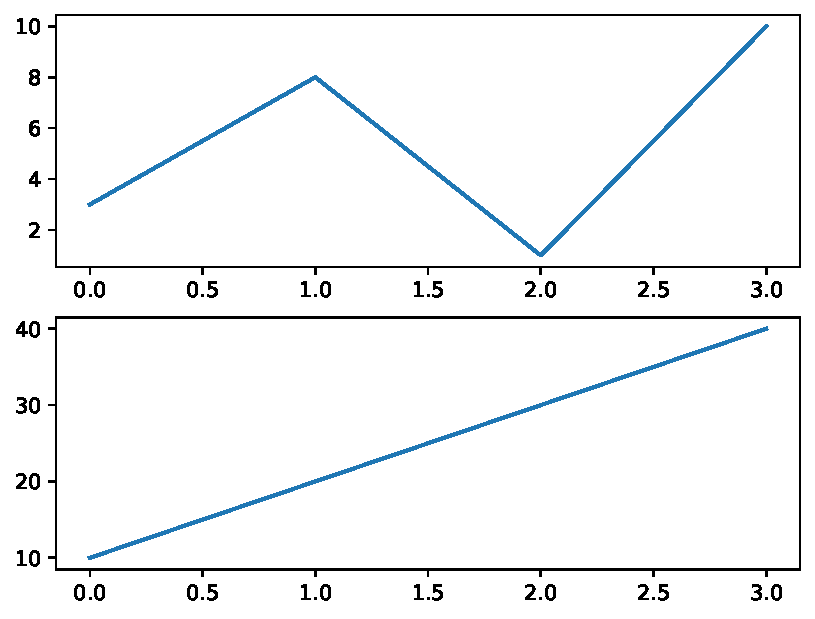
\includegraphics[scale=0.6]{img/grafica1032.pdf}
\end{figure}
\end{code}

Puede dibujar tantos gráficos como quiera en una figura, simplemente
describa el número de filas, columnas y el índice del gráfico.

\begin{code} Dibuje 6 gráficos.

\begin{Shaded}
\begin{Highlighting}[]
\ImportTok{import}\NormalTok{ matplotlib.pyplot }\ImportTok{as}\NormalTok{ plt}
\ImportTok{import}\NormalTok{ numpy }\ImportTok{as}\NormalTok{ np}

\NormalTok{x }\OperatorTok{=}\NormalTok{ np.array([}\DecValTok{0}\NormalTok{, }\DecValTok{1}\NormalTok{, }\DecValTok{2}\NormalTok{, }\DecValTok{3}\NormalTok{])}
\NormalTok{y }\OperatorTok{=}\NormalTok{ np.array([}\DecValTok{3}\NormalTok{, }\DecValTok{8}\NormalTok{, }\DecValTok{1}\NormalTok{, }\DecValTok{10}\NormalTok{])}

\NormalTok{plt.subplot(}\DecValTok{2}\NormalTok{, }\DecValTok{3}\NormalTok{, }\DecValTok{1}\NormalTok{)}
\NormalTok{plt.plot(x,y)}

\NormalTok{x }\OperatorTok{=}\NormalTok{ np.array([}\DecValTok{0}\NormalTok{, }\DecValTok{1}\NormalTok{, }\DecValTok{2}\NormalTok{, }\DecValTok{3}\NormalTok{])}
\NormalTok{y }\OperatorTok{=}\NormalTok{ np.array([}\DecValTok{10}\NormalTok{, }\DecValTok{20}\NormalTok{, }\DecValTok{30}\NormalTok{, }\DecValTok{40}\NormalTok{])}

\NormalTok{plt.subplot(}\DecValTok{2}\NormalTok{, }\DecValTok{3}\NormalTok{, }\DecValTok{2}\NormalTok{)}
\NormalTok{plt.plot(x,y)}

\NormalTok{x }\OperatorTok{=}\NormalTok{ np.array([}\DecValTok{0}\NormalTok{, }\DecValTok{1}\NormalTok{, }\DecValTok{2}\NormalTok{, }\DecValTok{3}\NormalTok{])}
\NormalTok{y }\OperatorTok{=}\NormalTok{ np.array([}\DecValTok{3}\NormalTok{, }\DecValTok{8}\NormalTok{, }\DecValTok{1}\NormalTok{, }\DecValTok{10}\NormalTok{])}

\NormalTok{plt.subplot(}\DecValTok{2}\NormalTok{, }\DecValTok{3}\NormalTok{, }\DecValTok{3}\NormalTok{)}
\NormalTok{plt.plot(x,y)}

\NormalTok{x }\OperatorTok{=}\NormalTok{ np.array([}\DecValTok{0}\NormalTok{, }\DecValTok{1}\NormalTok{, }\DecValTok{2}\NormalTok{, }\DecValTok{3}\NormalTok{])}
\NormalTok{y }\OperatorTok{=}\NormalTok{ np.array([}\DecValTok{10}\NormalTok{, }\DecValTok{20}\NormalTok{, }\DecValTok{30}\NormalTok{, }\DecValTok{40}\NormalTok{])}

\NormalTok{plt.subplot(}\DecValTok{2}\NormalTok{, }\DecValTok{3}\NormalTok{, }\DecValTok{4}\NormalTok{)}
\NormalTok{plt.plot(x,y)}

\NormalTok{x }\OperatorTok{=}\NormalTok{ np.array([}\DecValTok{0}\NormalTok{, }\DecValTok{1}\NormalTok{, }\DecValTok{2}\NormalTok{, }\DecValTok{3}\NormalTok{])}
\NormalTok{y }\OperatorTok{=}\NormalTok{ np.array([}\DecValTok{3}\NormalTok{, }\DecValTok{8}\NormalTok{, }\DecValTok{1}\NormalTok{, }\DecValTok{10}\NormalTok{])}

\NormalTok{plt.subplot(}\DecValTok{2}\NormalTok{, }\DecValTok{3}\NormalTok{, }\DecValTok{5}\NormalTok{)}
\NormalTok{plt.plot(x,y)}

\NormalTok{x }\OperatorTok{=}\NormalTok{ np.array([}\DecValTok{0}\NormalTok{, }\DecValTok{1}\NormalTok{, }\DecValTok{2}\NormalTok{, }\DecValTok{3}\NormalTok{])}
\NormalTok{y }\OperatorTok{=}\NormalTok{ np.array([}\DecValTok{10}\NormalTok{, }\DecValTok{20}\NormalTok{, }\DecValTok{30}\NormalTok{, }\DecValTok{40}\NormalTok{])}

\NormalTok{plt.subplot(}\DecValTok{2}\NormalTok{, }\DecValTok{3}\NormalTok{, }\DecValTok{6}\NormalTok{)}
\NormalTok{plt.plot(x,y)}
\NormalTok{plt.show()}
\end{Highlighting}
\end{Shaded}

\begin{figure}
  \centering
  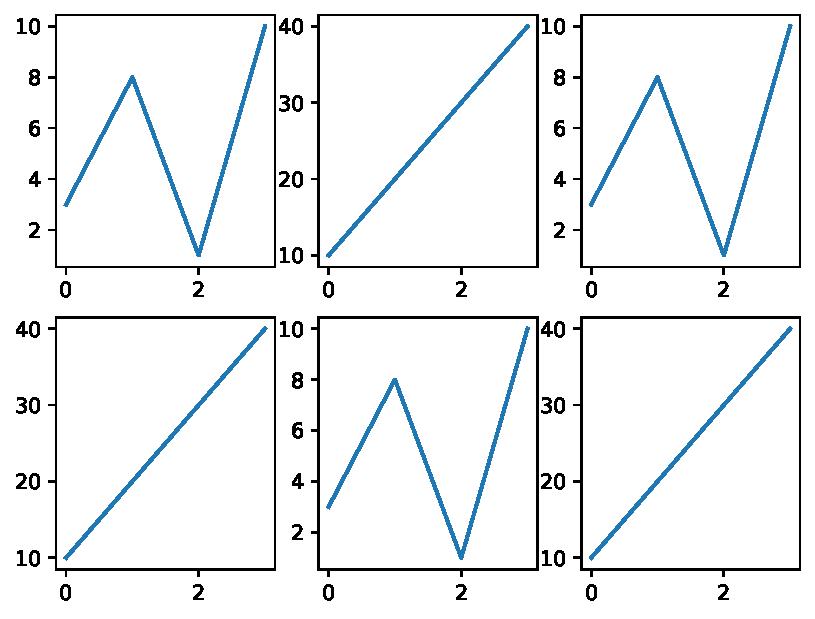
\includegraphics[scale=0.6]{img/grafica1033.pdf}
\end{figure}
\end{code}

\section{Título}

Puede agregar un título a cada gráfico con la función \texttt{title()}.

\begin{code} 2 parcelas, con títulos.

\begin{Shaded}
\begin{Highlighting}[]
\ImportTok{import}\NormalTok{ matplotlib.pyplot }\ImportTok{as}\NormalTok{ plt}
\ImportTok{import}\NormalTok{ numpy }\ImportTok{as}\NormalTok{ np}

\CommentTok{\#plot 1:}
\NormalTok{x }\OperatorTok{=}\NormalTok{ np.array([}\DecValTok{0}\NormalTok{, }\DecValTok{1}\NormalTok{, }\DecValTok{2}\NormalTok{, }\DecValTok{3}\NormalTok{])}
\NormalTok{y }\OperatorTok{=}\NormalTok{ np.array([}\DecValTok{3}\NormalTok{, }\DecValTok{8}\NormalTok{, }\DecValTok{1}\NormalTok{, }\DecValTok{10}\NormalTok{])}

\NormalTok{plt.subplot(}\DecValTok{1}\NormalTok{, }\DecValTok{2}\NormalTok{, }\DecValTok{1}\NormalTok{)}
\NormalTok{plt.plot(x,y)}
\NormalTok{plt.title(}\StringTok{"SALES"}\NormalTok{)}

\CommentTok{\#plot 2:}
\NormalTok{x }\OperatorTok{=}\NormalTok{ np.array([}\DecValTok{0}\NormalTok{, }\DecValTok{1}\NormalTok{, }\DecValTok{2}\NormalTok{, }\DecValTok{3}\NormalTok{])}
\NormalTok{y }\OperatorTok{=}\NormalTok{ np.array([}\DecValTok{10}\NormalTok{, }\DecValTok{20}\NormalTok{, }\DecValTok{30}\NormalTok{, }\DecValTok{40}\NormalTok{])}

\NormalTok{plt.subplot(}\DecValTok{1}\NormalTok{, }\DecValTok{2}\NormalTok{, }\DecValTok{2}\NormalTok{)}
\NormalTok{plt.plot(x,y)}
\NormalTok{plt.title(}\StringTok{"INCOME"}\NormalTok{)}

\NormalTok{plt.show()}
\end{Highlighting}
\end{Shaded}

\begin{figure}
  \centering
  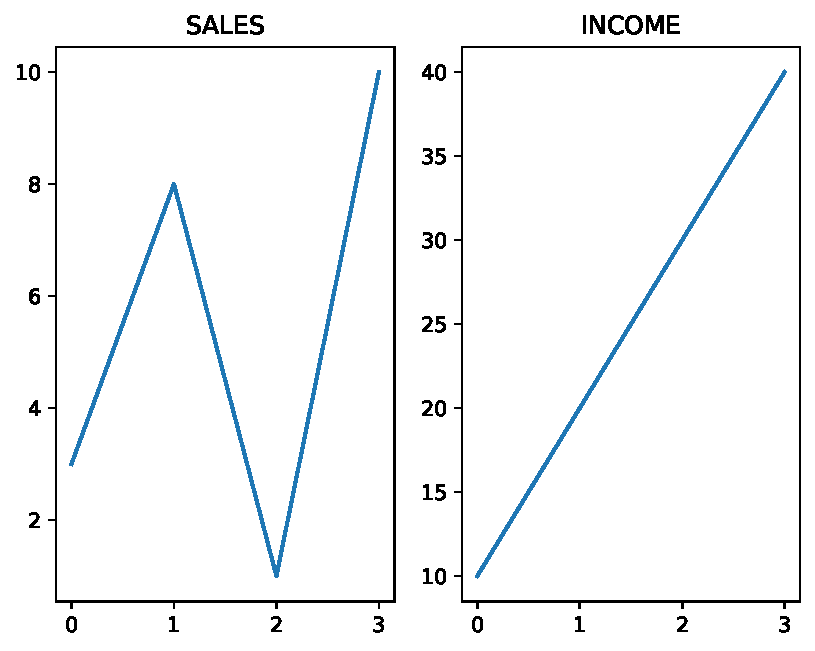
\includegraphics[scale=0.6]{img/grafica1034.pdf}
\end{figure}
\end{code}

\section{Súper título}

Puede agregar un título a toda la figura con la función
\texttt{suptitle()}.

\begin{code} Añade un título para toda la figura.

\begin{Shaded}
\begin{Highlighting}[]
\ImportTok{import}\NormalTok{ matplotlib.pyplot }\ImportTok{as}\NormalTok{ plt}
\ImportTok{import}\NormalTok{ numpy }\ImportTok{as}\NormalTok{ np}

\CommentTok{\#plot 1:}
\NormalTok{x }\OperatorTok{=}\NormalTok{ np.array([}\DecValTok{0}\NormalTok{, }\DecValTok{1}\NormalTok{, }\DecValTok{2}\NormalTok{, }\DecValTok{3}\NormalTok{])}
\NormalTok{y }\OperatorTok{=}\NormalTok{ np.array([}\DecValTok{3}\NormalTok{, }\DecValTok{8}\NormalTok{, }\DecValTok{1}\NormalTok{, }\DecValTok{10}\NormalTok{])}

\NormalTok{plt.subplot(}\DecValTok{1}\NormalTok{, }\DecValTok{2}\NormalTok{, }\DecValTok{1}\NormalTok{)}
\NormalTok{plt.plot(x,y)}
\NormalTok{plt.title(}\StringTok{"SALES"}\NormalTok{)}

\CommentTok{\#plot 2:}
\NormalTok{x }\OperatorTok{=}\NormalTok{ np.array([}\DecValTok{0}\NormalTok{, }\DecValTok{1}\NormalTok{, }\DecValTok{2}\NormalTok{, }\DecValTok{3}\NormalTok{])}
\NormalTok{y }\OperatorTok{=}\NormalTok{ np.array([}\DecValTok{10}\NormalTok{, }\DecValTok{20}\NormalTok{, }\DecValTok{30}\NormalTok{, }\DecValTok{40}\NormalTok{])}

\NormalTok{plt.subplot(}\DecValTok{1}\NormalTok{, }\DecValTok{2}\NormalTok{, }\DecValTok{2}\NormalTok{)}
\NormalTok{plt.plot(x,y)}
\NormalTok{plt.title(}\StringTok{"INCOME"}\NormalTok{)}

\NormalTok{plt.suptitle(}\StringTok{"MY SHOP"}\NormalTok{)}
\NormalTok{plt.show()}
\end{Highlighting}
\end{Shaded}

\begin{figure}
  \centering
  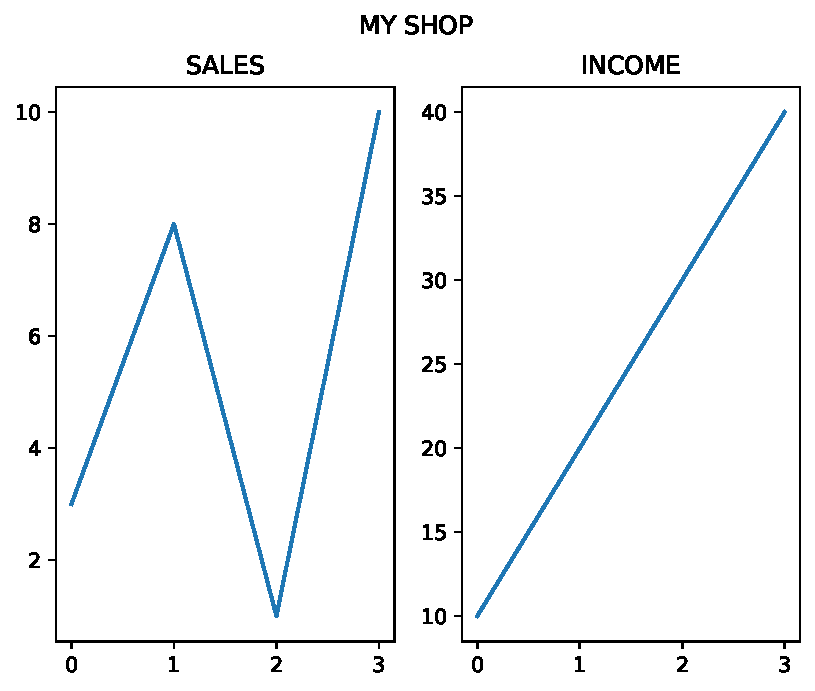
\includegraphics[scale=0.6]{img/grafica1035.pdf}
\end{figure}
\end{code}

\section{Gráficos de dispersión}

Con \texttt{Pyplot}, puede utilizar la función \texttt{scatter()} para
dibujar un diagrama de dispersión.

La función \texttt{scatter()} traza un punto para cada observación.
Necesita dos matrices de la misma longitud, una para los valores del eje
\(x\) y otra para los valores del eje \(y\).

\begin{code} Un diagrama de dispersión simple.

\begin{Shaded}
\begin{Highlighting}[]
\ImportTok{import}\NormalTok{ matplotlib.pyplot }\ImportTok{as}\NormalTok{ plt}
\ImportTok{import}\NormalTok{ numpy }\ImportTok{as}\NormalTok{ np}

\NormalTok{x }\OperatorTok{=}\NormalTok{ np.array([}\DecValTok{5}\NormalTok{,}\DecValTok{7}\NormalTok{,}\DecValTok{8}\NormalTok{,}\DecValTok{7}\NormalTok{,}\DecValTok{2}\NormalTok{,}\DecValTok{17}\NormalTok{,}\DecValTok{2}\NormalTok{,}\DecValTok{9}\NormalTok{,}\DecValTok{4}\NormalTok{,}\DecValTok{11}\NormalTok{,}\DecValTok{12}\NormalTok{,}\DecValTok{9}\NormalTok{,}\DecValTok{6}\NormalTok{])}
\NormalTok{y }\OperatorTok{=}\NormalTok{ np.array([}\DecValTok{99}\NormalTok{,}\DecValTok{86}\NormalTok{,}\DecValTok{87}\NormalTok{,}\DecValTok{88}\NormalTok{,}\DecValTok{111}\NormalTok{,}\DecValTok{86}\NormalTok{,}\DecValTok{103}\NormalTok{,}\DecValTok{87}\NormalTok{,}\DecValTok{94}\NormalTok{,}\DecValTok{78}\NormalTok{,}\DecValTok{77}\NormalTok{,}\DecValTok{85}\NormalTok{,}\DecValTok{86}\NormalTok{])}

\NormalTok{plt.scatter(x, y)}
\NormalTok{plt.show()}
\end{Highlighting}
\end{Shaded}

\begin{figure}
  \centering
  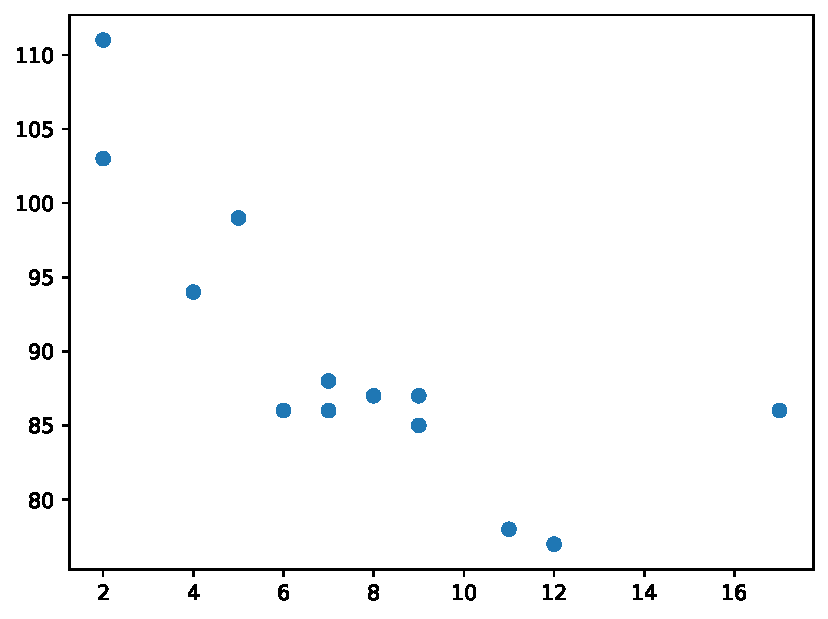
\includegraphics[scale=0.6]{img/grafica1036.pdf}
\end{figure}
\end{code}

La observación en el ejemplo anterior es el resultado de 13 automóviles.

El eje \(x\) muestra la antigüedad del coche y el eje \(y\) muestra la
velocidad del automóvil cuando pasa.

¿Existe alguna relación entre las observaciones?. Parece que cuanto más
nuevo es el coche, más rápido va, pero eso podría ser una coincidencia,
después de todo sólo registramos 13 coches.

\section{Comparar gráficos}

En el ejemplo anterior, parece haber una relación entre la velocidad y
la edad, pero ¿qué pasa si graficamos también las observaciones de otro
día? ¿El diagrama de dispersión nos dirá algo más?

\begin{code} Dibuje dos gráficos en la misma figura.

\begin{Shaded}
\begin{Highlighting}[]
\ImportTok{import}\NormalTok{ matplotlib.pyplot }\ImportTok{as}\NormalTok{ plt}
\ImportTok{import}\NormalTok{ numpy }\ImportTok{as}\NormalTok{ np}

\CommentTok{\#day one, the age and speed of 13 cars:}
\NormalTok{x }\OperatorTok{=}\NormalTok{ np.array([}\DecValTok{5}\NormalTok{,}\DecValTok{7}\NormalTok{,}\DecValTok{8}\NormalTok{,}\DecValTok{7}\NormalTok{,}\DecValTok{2}\NormalTok{,}\DecValTok{17}\NormalTok{,}\DecValTok{2}\NormalTok{,}\DecValTok{9}\NormalTok{,}\DecValTok{4}\NormalTok{,}\DecValTok{11}\NormalTok{,}\DecValTok{12}\NormalTok{,}\DecValTok{9}\NormalTok{,}\DecValTok{6}\NormalTok{])}
\NormalTok{y }\OperatorTok{=}\NormalTok{ np.array([}\DecValTok{99}\NormalTok{,}\DecValTok{86}\NormalTok{,}\DecValTok{87}\NormalTok{,}\DecValTok{88}\NormalTok{,}\DecValTok{111}\NormalTok{,}\DecValTok{86}\NormalTok{,}\DecValTok{103}\NormalTok{,}\DecValTok{87}\NormalTok{,}\DecValTok{94}\NormalTok{,}\DecValTok{78}\NormalTok{,}\DecValTok{77}\NormalTok{,}\DecValTok{85}\NormalTok{,}\DecValTok{86}\NormalTok{])}
\NormalTok{plt.scatter(x, y)}

\CommentTok{\#day two, the age and speed of 15 cars:}
\NormalTok{x }\OperatorTok{=}\NormalTok{ np.array([}\DecValTok{2}\NormalTok{,}\DecValTok{2}\NormalTok{,}\DecValTok{8}\NormalTok{,}\DecValTok{1}\NormalTok{,}\DecValTok{15}\NormalTok{,}\DecValTok{8}\NormalTok{,}\DecValTok{12}\NormalTok{,}\DecValTok{9}\NormalTok{,}\DecValTok{7}\NormalTok{,}\DecValTok{3}\NormalTok{,}\DecValTok{11}\NormalTok{,}\DecValTok{4}\NormalTok{,}\DecValTok{7}\NormalTok{,}\DecValTok{14}\NormalTok{,}\DecValTok{12}\NormalTok{])}
\NormalTok{y }\OperatorTok{=}\NormalTok{ np.array([}\DecValTok{100}\NormalTok{,}\DecValTok{105}\NormalTok{,}\DecValTok{84}\NormalTok{,}\DecValTok{105}\NormalTok{,}\DecValTok{90}\NormalTok{,}\DecValTok{99}\NormalTok{,}\DecValTok{90}\NormalTok{,}\DecValTok{95}\NormalTok{,}\DecValTok{94}\NormalTok{,}\DecValTok{100}\NormalTok{,}\DecValTok{79}\NormalTok{,}\DecValTok{112}\NormalTok{,}\DecValTok{91}\NormalTok{,}\DecValTok{80}\NormalTok{,}\DecValTok{85}\NormalTok{])}
\NormalTok{plt.scatter(x, y)}

\NormalTok{plt.show()}
\end{Highlighting}
\end{Shaded}

\begin{figure}
  \centering
  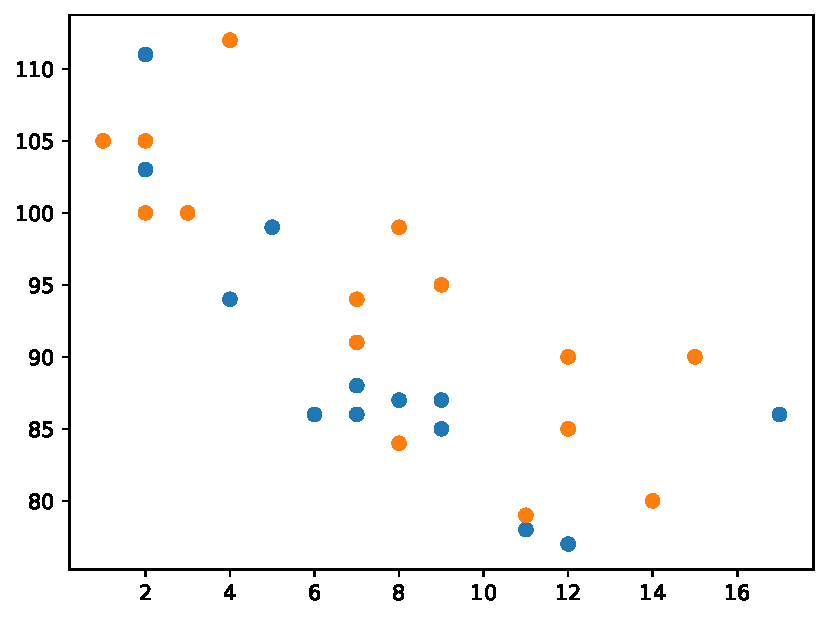
\includegraphics[scale=0.6]{img/grafica1037.pdf}
\end{figure}
\end{code}

\textbf{Nota}: Los dos gráficos están representados con dos colores
diferentes, por defecto azul y naranja.

Comparando ambos gráficos, creo que es seguro decir que ambos nos llevan
a la misma conclusión: cuanto más nuevo es el coche, más rápido va.

\section{Colores}

Puede establecer su propio color para cada gráfico de dispersión con
\texttt{color} o el argumento \texttt{c}.

\begin{code} Establezca su propio color de marcadores.

\begin{Shaded}
\begin{Highlighting}[]
\ImportTok{import}\NormalTok{ matplotlib.pyplot }\ImportTok{as}\NormalTok{ plt}
\ImportTok{import}\NormalTok{ numpy }\ImportTok{as}\NormalTok{ np}

\NormalTok{x }\OperatorTok{=}\NormalTok{ np.array([}\DecValTok{5}\NormalTok{,}\DecValTok{7}\NormalTok{,}\DecValTok{8}\NormalTok{,}\DecValTok{7}\NormalTok{,}\DecValTok{2}\NormalTok{,}\DecValTok{17}\NormalTok{,}\DecValTok{2}\NormalTok{,}\DecValTok{9}\NormalTok{,}\DecValTok{4}\NormalTok{,}\DecValTok{11}\NormalTok{,}\DecValTok{12}\NormalTok{,}\DecValTok{9}\NormalTok{,}\DecValTok{6}\NormalTok{])}
\NormalTok{y }\OperatorTok{=}\NormalTok{ np.array([}\DecValTok{99}\NormalTok{,}\DecValTok{86}\NormalTok{,}\DecValTok{87}\NormalTok{,}\DecValTok{88}\NormalTok{,}\DecValTok{111}\NormalTok{,}\DecValTok{86}\NormalTok{,}\DecValTok{103}\NormalTok{,}\DecValTok{87}\NormalTok{,}\DecValTok{94}\NormalTok{,}\DecValTok{78}\NormalTok{,}\DecValTok{77}\NormalTok{,}\DecValTok{85}\NormalTok{,}\DecValTok{86}\NormalTok{])}
\NormalTok{plt.scatter(x, y, color }\OperatorTok{=} \StringTok{\textquotesingle{}hotpink\textquotesingle{}}\NormalTok{)}

\NormalTok{x }\OperatorTok{=}\NormalTok{ np.array([}\DecValTok{2}\NormalTok{,}\DecValTok{2}\NormalTok{,}\DecValTok{8}\NormalTok{,}\DecValTok{1}\NormalTok{,}\DecValTok{15}\NormalTok{,}\DecValTok{8}\NormalTok{,}\DecValTok{12}\NormalTok{,}\DecValTok{9}\NormalTok{,}\DecValTok{7}\NormalTok{,}\DecValTok{3}\NormalTok{,}\DecValTok{11}\NormalTok{,}\DecValTok{4}\NormalTok{,}\DecValTok{7}\NormalTok{,}\DecValTok{14}\NormalTok{,}\DecValTok{12}\NormalTok{])}
\NormalTok{y }\OperatorTok{=}\NormalTok{ np.array([}\DecValTok{100}\NormalTok{,}\DecValTok{105}\NormalTok{,}\DecValTok{84}\NormalTok{,}\DecValTok{105}\NormalTok{,}\DecValTok{90}\NormalTok{,}\DecValTok{99}\NormalTok{,}\DecValTok{90}\NormalTok{,}\DecValTok{95}\NormalTok{,}\DecValTok{94}\NormalTok{,}\DecValTok{100}\NormalTok{,}\DecValTok{79}\NormalTok{,}\DecValTok{112}\NormalTok{,}\DecValTok{91}\NormalTok{,}\DecValTok{80}\NormalTok{,}\DecValTok{85}\NormalTok{])}
\NormalTok{plt.scatter(x, y, color }\OperatorTok{=} \StringTok{\textquotesingle{}\#88c999\textquotesingle{}}\NormalTok{)}

\NormalTok{plt.show()}
\end{Highlighting}
\end{Shaded}

\begin{figure}
  \centering
  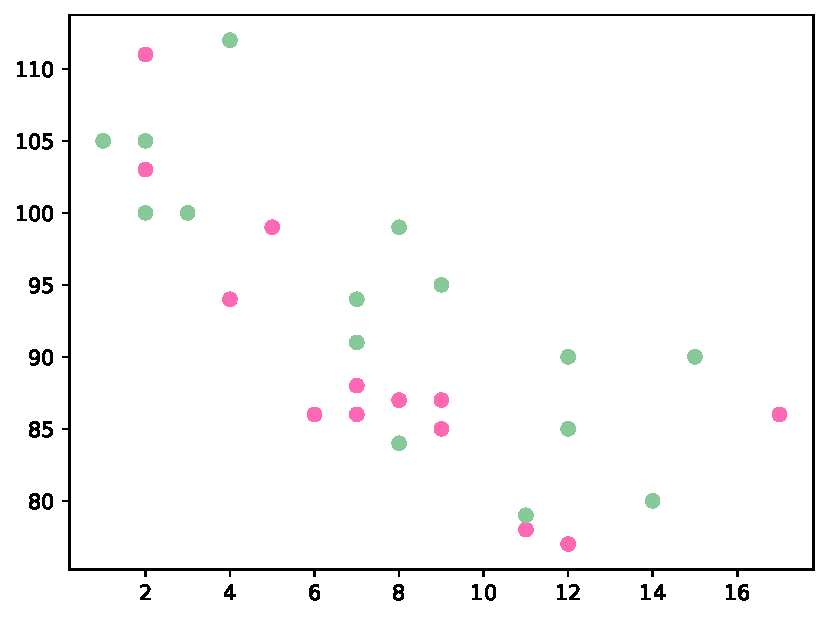
\includegraphics[scale=0.6]{img/grafica1038.pdf}
\end{figure}
\end{code}

\section{Colorear cada punto}

Es posible establecer un color específico para cada punto utilizando una
matriz de colores como valor para el cargumento.

\textbf{Nota}: No puede usar el argumento \texttt{color} para esto, solo
el argumento \texttt{c}.\\

\begin{code} Colorear puntos de dispersión.
\begin{Shaded}
\begin{Highlighting}[]
\ImportTok{import}\NormalTok{ matplotlib.pyplot }\ImportTok{as}\NormalTok{ plt}
\ImportTok{import}\NormalTok{ numpy }\ImportTok{as}\NormalTok{ np}

\NormalTok{x }\OperatorTok{=}\NormalTok{ np.array([}\DecValTok{5}\NormalTok{,}\DecValTok{7}\NormalTok{,}\DecValTok{8}\NormalTok{,}\DecValTok{7}\NormalTok{,}\DecValTok{2}\NormalTok{,}\DecValTok{17}\NormalTok{,}\DecValTok{2}\NormalTok{,}\DecValTok{9}\NormalTok{,}\DecValTok{4}\NormalTok{,}\DecValTok{11}\NormalTok{,}\DecValTok{12}\NormalTok{,}\DecValTok{9}\NormalTok{,}\DecValTok{6}\NormalTok{])}
\NormalTok{y }\OperatorTok{=}\NormalTok{ np.array([}\DecValTok{99}\NormalTok{,}\DecValTok{86}\NormalTok{,}\DecValTok{87}\NormalTok{,}\DecValTok{88}\NormalTok{,}\DecValTok{111}\NormalTok{,}\DecValTok{86}\NormalTok{,}\DecValTok{103}\NormalTok{,}\DecValTok{87}\NormalTok{,}\DecValTok{94}\NormalTok{,}\DecValTok{78}\NormalTok{,}\DecValTok{77}\NormalTok{,}\DecValTok{85}\NormalTok{,}\DecValTok{86}\NormalTok{])}
\NormalTok{colors }\OperatorTok{=}\NormalTok{ np.array([}\StringTok{"red"}\NormalTok{,}\StringTok{"green"}\NormalTok{,}\StringTok{"blue"}\NormalTok{,}\StringTok{"yellow"}\NormalTok{,}\StringTok{"pink"}\NormalTok{,}\StringTok{"black"}\NormalTok{,}\StringTok{"orange"}\NormalTok{,}\StringTok{"purple"}\NormalTok{,}
    \StringTok{"beige"}\NormalTok{,}\StringTok{"brown"}\NormalTok{,}\StringTok{"gray"}\NormalTok{,}\StringTok{"cyan"}\NormalTok{,}\StringTok{"magenta"}\NormalTok{])}

\NormalTok{plt.scatter(x, y, c}\OperatorTok{=}\NormalTok{colors)}

\NormalTok{plt.show()}
\end{Highlighting}
\end{Shaded}

\begin{figure}
  \centering
  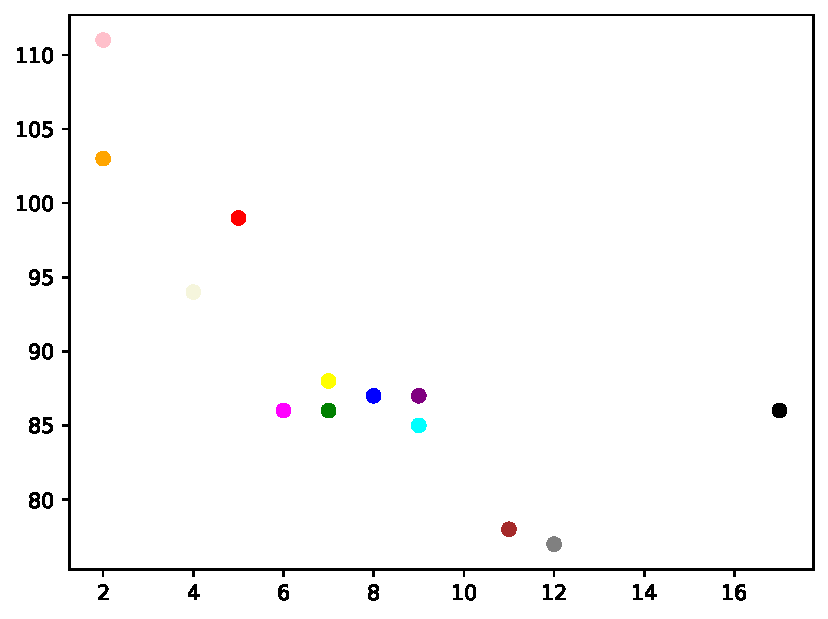
\includegraphics[scale=0.6]{img/grafica1039.pdf}
\end{figure}
\end{code}

\section{Mapa de colores}

El módulo \texttt{Matplotlib} tiene varios mapas de colores disponibles.

Un mapa de colores es una lista de colores, donde cada color tiene un
valor que varía de 0 a 100.

A continuación se muestra un ejemplo de un mapa de colores:
\begin{figure}
  \centering
  
\includegraphics[scale=0.6]{img/img_colorbar.png}
\end{figure}


Este mapa de colores se llama
\emph{\textquotesingle viridis\textquotesingle{}} y como puedes ver,
varía desde 0, que es un color púrpura, hasta 100, que es un color
amarillo.

\subsubsection{Cómo utilizar el mapa de colores}

Puede especificar el mapa de colores con el argumento de palabra clave
\texttt{cmap}, en este caso
\emph{\textquotesingle viridis\textquotesingle{}} que es uno de los
mapas de colores integrados disponibles en \texttt{Matplotlib}.

Además, debes crear una matriz con valores (de 0 a 100), un valor para
cada punto en el diagrama de dispersión.\\

\begin{code} Cree una matriz de colores y especifique un mapa de
colores en el gráfico de dispersión.

\begin{Shaded}
\begin{Highlighting}[]
\ImportTok{import}\NormalTok{ matplotlib.pyplot }\ImportTok{as}\NormalTok{ plt}
\ImportTok{import}\NormalTok{ numpy }\ImportTok{as}\NormalTok{ np}

\NormalTok{x }\OperatorTok{=}\NormalTok{ np.array([}\DecValTok{5}\NormalTok{,}\DecValTok{7}\NormalTok{,}\DecValTok{8}\NormalTok{,}\DecValTok{7}\NormalTok{,}\DecValTok{2}\NormalTok{,}\DecValTok{17}\NormalTok{,}\DecValTok{2}\NormalTok{,}\DecValTok{9}\NormalTok{,}\DecValTok{4}\NormalTok{,}\DecValTok{11}\NormalTok{,}\DecValTok{12}\NormalTok{,}\DecValTok{9}\NormalTok{,}\DecValTok{6}\NormalTok{])}
\NormalTok{y }\OperatorTok{=}\NormalTok{ np.array([}\DecValTok{99}\NormalTok{,}\DecValTok{86}\NormalTok{,}\DecValTok{87}\NormalTok{,}\DecValTok{88}\NormalTok{,}\DecValTok{111}\NormalTok{,}\DecValTok{86}\NormalTok{,}\DecValTok{103}\NormalTok{,}\DecValTok{87}\NormalTok{,}\DecValTok{94}\NormalTok{,}\DecValTok{78}\NormalTok{,}\DecValTok{77}\NormalTok{,}\DecValTok{85}\NormalTok{,}\DecValTok{86}\NormalTok{])}
\NormalTok{colors }\OperatorTok{=}\NormalTok{ np.array([}\DecValTok{0}\NormalTok{, }\DecValTok{10}\NormalTok{, }\DecValTok{20}\NormalTok{, }\DecValTok{30}\NormalTok{, }\DecValTok{40}\NormalTok{, }\DecValTok{45}\NormalTok{, }\DecValTok{50}\NormalTok{, }\DecValTok{55}\NormalTok{, }\DecValTok{60}\NormalTok{, }\DecValTok{70}\NormalTok{, }\DecValTok{80}\NormalTok{, }\DecValTok{90}\NormalTok{, }\DecValTok{100}\NormalTok{])}

\NormalTok{plt.scatter(x, y, c}\OperatorTok{=}\NormalTok{colors, cmap}\OperatorTok{=}\StringTok{\textquotesingle{}viridis\textquotesingle{}}\NormalTok{)}

\NormalTok{plt.show()}
\end{Highlighting}
\end{Shaded}

\begin{figure}
  \centering
  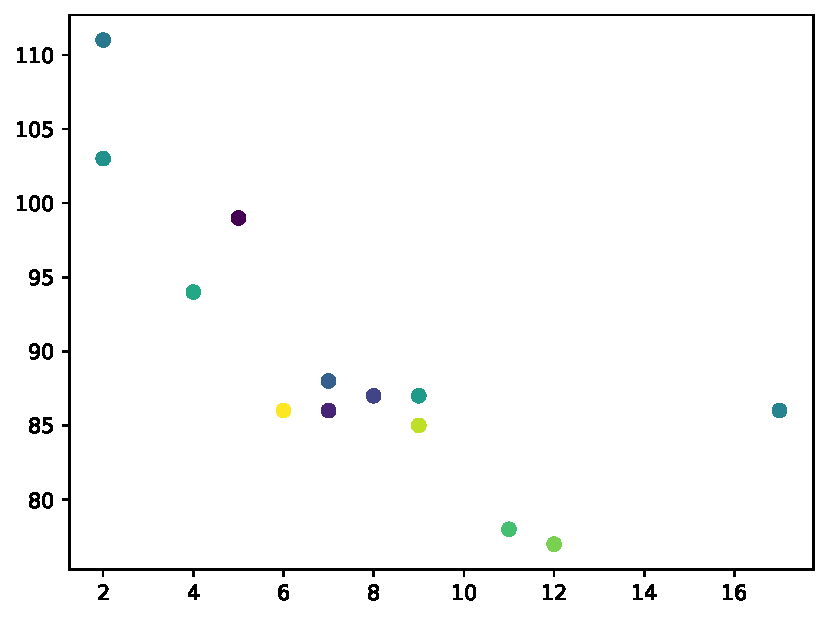
\includegraphics[scale=0.6]{img/grafica1040.pdf}
\end{figure}
\end{code}

Puede incluir el mapa de colores en el dibujo incluyendo la declaración \texttt{plt.colorbar()}.\\

\begin{code} Incluya el mapa de colores real.

\begin{Shaded}
\begin{Highlighting}[]
\ImportTok{import}\NormalTok{ matplotlib.pyplot }\ImportTok{as}\NormalTok{ plt}
\ImportTok{import}\NormalTok{ numpy }\ImportTok{as}\NormalTok{ np}

\NormalTok{x }\OperatorTok{=}\NormalTok{ np.array([}\DecValTok{5}\NormalTok{,}\DecValTok{7}\NormalTok{,}\DecValTok{8}\NormalTok{,}\DecValTok{7}\NormalTok{,}\DecValTok{2}\NormalTok{,}\DecValTok{17}\NormalTok{,}\DecValTok{2}\NormalTok{,}\DecValTok{9}\NormalTok{,}\DecValTok{4}\NormalTok{,}\DecValTok{11}\NormalTok{,}\DecValTok{12}\NormalTok{,}\DecValTok{9}\NormalTok{,}\DecValTok{6}\NormalTok{])}
\NormalTok{y }\OperatorTok{=}\NormalTok{ np.array([}\DecValTok{99}\NormalTok{,}\DecValTok{86}\NormalTok{,}\DecValTok{87}\NormalTok{,}\DecValTok{88}\NormalTok{,}\DecValTok{111}\NormalTok{,}\DecValTok{86}\NormalTok{,}\DecValTok{103}\NormalTok{,}\DecValTok{87}\NormalTok{,}\DecValTok{94}\NormalTok{,}\DecValTok{78}\NormalTok{,}\DecValTok{77}\NormalTok{,}\DecValTok{85}\NormalTok{,}\DecValTok{86}\NormalTok{])}
\NormalTok{colors }\OperatorTok{=}\NormalTok{ np.array([}\DecValTok{0}\NormalTok{, }\DecValTok{10}\NormalTok{, }\DecValTok{20}\NormalTok{, }\DecValTok{30}\NormalTok{, }\DecValTok{40}\NormalTok{, }\DecValTok{45}\NormalTok{, }\DecValTok{50}\NormalTok{, }\DecValTok{55}\NormalTok{, }\DecValTok{60}\NormalTok{, }\DecValTok{70}\NormalTok{, }\DecValTok{80}\NormalTok{, }\DecValTok{90}\NormalTok{, }\DecValTok{100}\NormalTok{])}

\NormalTok{plt.scatter(x, y, c}\OperatorTok{=}\NormalTok{colors, cmap}\OperatorTok{=}\StringTok{\textquotesingle{}gist\_rainbow\textquotesingle{}}\NormalTok{)}

\NormalTok{plt.colorbar()}

\NormalTok{plt.show()}
\end{Highlighting}
\end{Shaded}

\begin{figure}
  \centering
  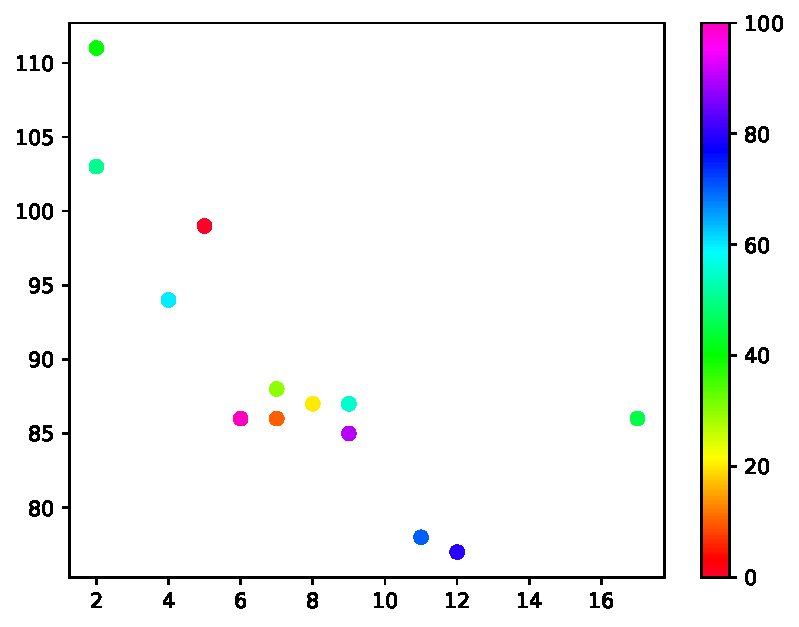
\includegraphics[scale=0.6]{img/grafica1041.pdf}
\end{figure}
\end{code}

\section{Mapas de colores disponibles}

Puede elegir cualquiera de los
\href{https://matplotlib.org/stable/users/explain/colors/colormaps.html}{mapas
de colores incorporados}.

\begin{Shaded}
\begin{Highlighting}[]
\ImportTok{from}\NormalTok{ matplotlib }\ImportTok{import}\NormalTok{ colormaps}
\BuiltInTok{list}\NormalTok{(colormaps)}
\end{Highlighting}
\end{Shaded}

\begin{verbatim}
['magma',
 'inferno',
 'plasma',
 'viridis',
 'cividis',
 'twilight',
 'twilight_shifted',
 'turbo',
 'Blues',
 'BrBG',
 'BuGn',
 'BuPu',
 'CMRmap',
 'GnBu',
 'Greens',
 'Greys',
 'OrRd',
 'Oranges',
 'PRGn',
 'PiYG',
 'PuBu',
 'PuBuGn',
 'PuOr',
 'PuRd',
 'Purples',
 'RdBu',
 'RdGy',
 'RdPu',
 'RdYlBu',
 'RdYlGn',
 'Reds',
 'Spectral',
 'Wistia',
 'YlGn',
 'YlGnBu',
 'YlOrBr',
 'YlOrRd',
 'afmhot',
 'autumn',
 'binary',
 'bone',
 'brg',
 'bwr',
 'cool',
 'coolwarm',
 'copper',
 'cubehelix',
 'flag',
 'gist_earth',
 'gist_gray',
 'gist_heat',
 'gist_ncar',
 'gist_rainbow',
 'gist_stern',
 'gist_yarg',
 'gnuplot',
 'gnuplot2',
 'gray',
 'hot',
 'hsv',
 'jet',
 'nipy_spectral',
 'ocean',
 'pink',
 'prism',
 'rainbow',
 'seismic',
 'spring',
 'summer',
 'terrain',
 'winter',
 'Accent',
 'Dark2',
 'Paired',
 'Pastel1',
 'Pastel2',
 'Set1',
 'Set2',
 'Set3',
 'tab10',
 'tab20',
 'tab20b',
 'tab20c',
 'grey',
 'gist_grey',
 'gist_yerg',
 'Grays',
 'magma_r',
 'inferno_r',
 'plasma_r',
 'viridis_r',
 'cividis_r',
 'twilight_r',
 'twilight_shifted_r',
 'turbo_r',
 'Blues_r',
 'BrBG_r',
 'BuGn_r',
 'BuPu_r',
 'CMRmap_r',
 'GnBu_r',
 'Greens_r',
 'Greys_r',
 'OrRd_r',
 'Oranges_r',
 'PRGn_r',
 'PiYG_r',
 'PuBu_r',
 'PuBuGn_r',
 'PuOr_r',
 'PuRd_r',
 'Purples_r',
 'RdBu_r',
 'RdGy_r',
 'RdPu_r',
 'RdYlBu_r',
 'RdYlGn_r',
 'Reds_r',
 'Spectral_r',
 'Wistia_r',
 'YlGn_r',
 'YlGnBu_r',
 'YlOrBr_r',
 'YlOrRd_r',
 'afmhot_r',
 'autumn_r',
 'binary_r',
 'bone_r',
 'brg_r',
 'bwr_r',
 'cool_r',
 'coolwarm_r',
 'copper_r',
 'cubehelix_r',
 'flag_r',
 'gist_earth_r',
 'gist_gray_r',
 'gist_heat_r',
 'gist_ncar_r',
 'gist_rainbow_r',
 'gist_stern_r',
 'gist_yarg_r',
 'gnuplot_r',
 'gnuplot2_r',
 'gray_r',
 'hot_r',
 'hsv_r',
 'jet_r',
 'nipy_spectral_r',
 'ocean_r',
 'pink_r',
 'prism_r',
 'rainbow_r',
 'seismic_r',
 'spring_r',
 'summer_r',
 'terrain_r',
 'winter_r',
 'Accent_r',
 'Dark2_r',
 'Paired_r',
 'Pastel1_r',
 'Pastel2_r',
 'Set1_r',
 'Set2_r',
 'Set3_r',
 'tab10_r',
 'tab20_r',
 'tab20b_r',
 'tab20c_r']
\end{verbatim}

\section{Tamaño}

Puede cambiar el tamaño de los puntos con el sargumento.

Al igual que con los colores, asegúrese de que la matriz de tamaños
tenga la misma longitud que las matrices de ejes \(x\) y \(y\).

\begin{code} Establezca su propio tamaño para los marcadores.

\begin{Shaded}
\begin{Highlighting}[]
\ImportTok{import}\NormalTok{ matplotlib.pyplot }\ImportTok{as}\NormalTok{ plt}
\ImportTok{import}\NormalTok{ numpy }\ImportTok{as}\NormalTok{ np}

\NormalTok{x }\OperatorTok{=}\NormalTok{ np.array([}\DecValTok{5}\NormalTok{,}\DecValTok{7}\NormalTok{,}\DecValTok{8}\NormalTok{,}\DecValTok{7}\NormalTok{,}\DecValTok{2}\NormalTok{,}\DecValTok{17}\NormalTok{,}\DecValTok{2}\NormalTok{,}\DecValTok{9}\NormalTok{,}\DecValTok{4}\NormalTok{,}\DecValTok{11}\NormalTok{,}\DecValTok{12}\NormalTok{,}\DecValTok{9}\NormalTok{,}\DecValTok{6}\NormalTok{])}
\NormalTok{y }\OperatorTok{=}\NormalTok{ np.array([}\DecValTok{99}\NormalTok{,}\DecValTok{86}\NormalTok{,}\DecValTok{87}\NormalTok{,}\DecValTok{88}\NormalTok{,}\DecValTok{111}\NormalTok{,}\DecValTok{86}\NormalTok{,}\DecValTok{103}\NormalTok{,}\DecValTok{87}\NormalTok{,}\DecValTok{94}\NormalTok{,}\DecValTok{78}\NormalTok{,}\DecValTok{77}\NormalTok{,}\DecValTok{85}\NormalTok{,}\DecValTok{86}\NormalTok{])}
\NormalTok{sizes }\OperatorTok{=}\NormalTok{ np.array([}\DecValTok{20}\NormalTok{,}\DecValTok{50}\NormalTok{,}\DecValTok{100}\NormalTok{,}\DecValTok{200}\NormalTok{,}\DecValTok{500}\NormalTok{,}\DecValTok{1000}\NormalTok{,}\DecValTok{60}\NormalTok{,}\DecValTok{90}\NormalTok{,}\DecValTok{10}\NormalTok{,}\DecValTok{300}\NormalTok{,}\DecValTok{600}\NormalTok{,}\DecValTok{800}\NormalTok{,}\DecValTok{75}\NormalTok{])}

\NormalTok{plt.scatter(x, y, s}\OperatorTok{=}\NormalTok{sizes)}
\NormalTok{plt.show()}
\end{Highlighting}
\end{Shaded}

\begin{figure}
  \centering
  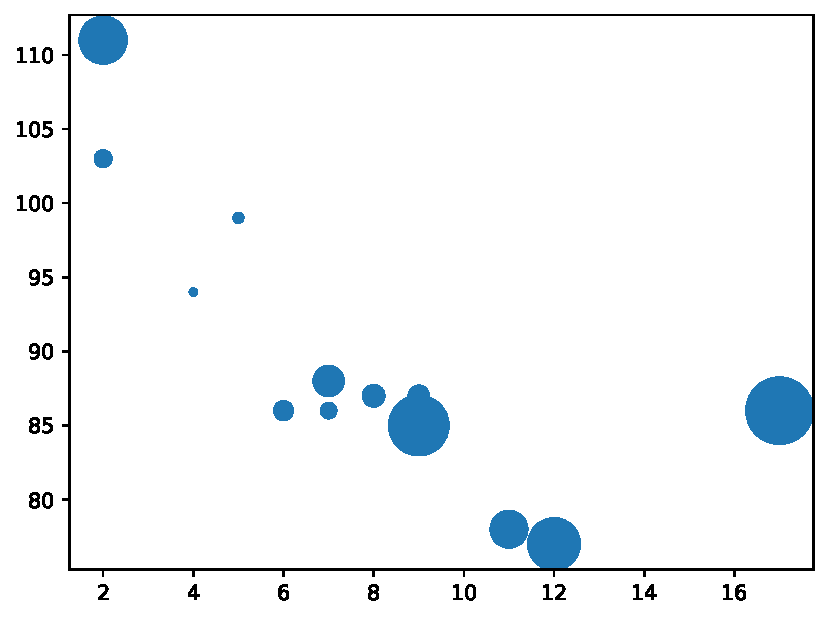
\includegraphics[scale=0.6]{img/grafica1042.pdf}
\end{figure}
\end{code}

\section{Transparencia}

Puede ajustar la transparencia de los puntos con el argumento \texttt{alpha}.

Al igual que con los colores, es posbile ajustar la transparencia a los
puntos individualmente, sólo asegúrese de que la matriz de tamaños tenga
la misma longitud que las matrices de ejes \(x\) y \(y\).\\

\begin{code} Establezca su propio tamaño para los marcadores.

\begin{Shaded}
\begin{Highlighting}[]
\ImportTok{import}\NormalTok{ matplotlib.pyplot }\ImportTok{as}\NormalTok{ plt}
\ImportTok{import}\NormalTok{ numpy }\ImportTok{as}\NormalTok{ np}

\NormalTok{x }\OperatorTok{=}\NormalTok{ np.array([}\DecValTok{5}\NormalTok{,}\DecValTok{7}\NormalTok{,}\DecValTok{8}\NormalTok{,}\DecValTok{7}\NormalTok{,}\DecValTok{2}\NormalTok{,}\DecValTok{17}\NormalTok{,}\DecValTok{2}\NormalTok{,}\DecValTok{9}\NormalTok{,}\DecValTok{4}\NormalTok{,}\DecValTok{11}\NormalTok{,}\DecValTok{12}\NormalTok{,}\DecValTok{9}\NormalTok{,}\DecValTok{6}\NormalTok{])}
\NormalTok{y }\OperatorTok{=}\NormalTok{ np.array([}\DecValTok{99}\NormalTok{,}\DecValTok{86}\NormalTok{,}\DecValTok{87}\NormalTok{,}\DecValTok{88}\NormalTok{,}\DecValTok{111}\NormalTok{,}\DecValTok{86}\NormalTok{,}\DecValTok{103}\NormalTok{,}\DecValTok{87}\NormalTok{,}\DecValTok{94}\NormalTok{,}\DecValTok{78}\NormalTok{,}\DecValTok{77}\NormalTok{,}\DecValTok{85}\NormalTok{,}\DecValTok{86}\NormalTok{])}
\NormalTok{sizes }\OperatorTok{=}\NormalTok{ np.array([}\DecValTok{20}\NormalTok{,}\DecValTok{50}\NormalTok{,}\DecValTok{100}\NormalTok{,}\DecValTok{200}\NormalTok{,}\DecValTok{500}\NormalTok{,}\DecValTok{1000}\NormalTok{,}\DecValTok{60}\NormalTok{,}\DecValTok{90}\NormalTok{,}\DecValTok{10}\NormalTok{,}\DecValTok{300}\NormalTok{,}\DecValTok{600}\NormalTok{,}\DecValTok{800}\NormalTok{,}\DecValTok{75}\NormalTok{])}
\NormalTok{transparency }\OperatorTok{=}\NormalTok{ np.array([}\FloatTok{0.1}\NormalTok{, }\FloatTok{0.2}\NormalTok{, }\FloatTok{0.3}\NormalTok{, }\FloatTok{0.4}\NormalTok{, }\FloatTok{0.5}\NormalTok{, }\FloatTok{0.6}\NormalTok{, }\FloatTok{0.7}\NormalTok{, }\FloatTok{0.8}\NormalTok{, }\FloatTok{0.9}\NormalTok{, }\DecValTok{1}\NormalTok{, }\FloatTok{0.9}\NormalTok{, }\FloatTok{0.8}\NormalTok{, }\FloatTok{0.3}\NormalTok{])}

\NormalTok{plt.scatter(x, y, s}\OperatorTok{=}\NormalTok{sizes, alpha}\OperatorTok{=}\NormalTok{transparency)}
\NormalTok{plt.show()}
\end{Highlighting}
\end{Shaded}

\begin{figure}
  \centering
  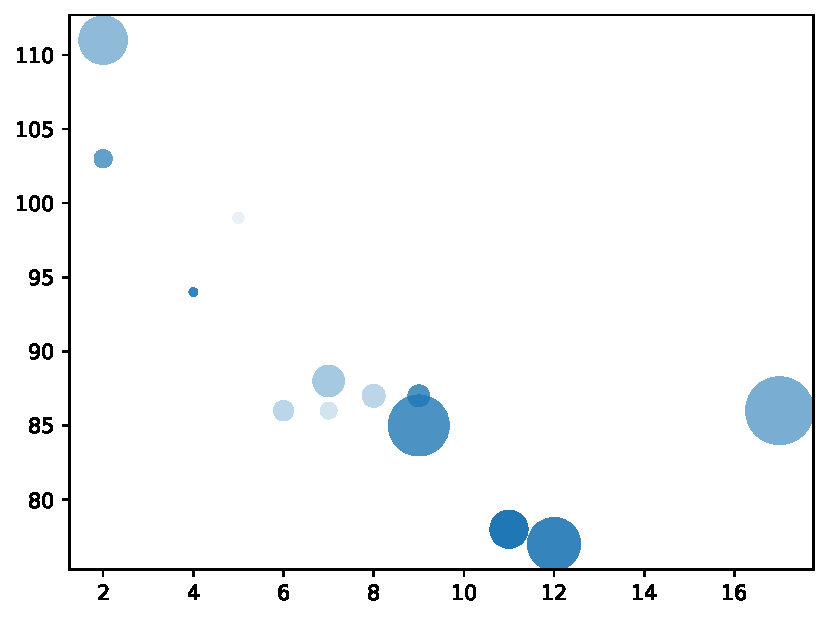
\includegraphics[scale=0.6]{img/grafica1043.pdf}
\end{figure}
\end{code}

\section{Combinar color, tamaño y alfa}

Se puede combinar un mapa de colores con diferentes tamaños de puntos.
Esto se visualiza mejor si los puntos son transparentes.\\

\begin{code} Crear matrices aleatorias con 100 valores para puntos \(x\), puntos \(y\), colores y tamaños.

\begin{Shaded}
\begin{Highlighting}[]
\ImportTok{import}\NormalTok{ matplotlib.pyplot }\ImportTok{as}\NormalTok{ plt}
\ImportTok{import}\NormalTok{ numpy }\ImportTok{as}\NormalTok{ np}

\NormalTok{x }\OperatorTok{=}\NormalTok{ np.random.randint(}\DecValTok{100}\NormalTok{, size}\OperatorTok{=}\NormalTok{(}\DecValTok{100}\NormalTok{))}
\NormalTok{y }\OperatorTok{=}\NormalTok{ np.random.randint(}\DecValTok{100}\NormalTok{, size}\OperatorTok{=}\NormalTok{(}\DecValTok{100}\NormalTok{))}
\NormalTok{colors }\OperatorTok{=}\NormalTok{ np.random.randint(}\DecValTok{100}\NormalTok{, size}\OperatorTok{=}\NormalTok{(}\DecValTok{100}\NormalTok{))}
\NormalTok{sizes }\OperatorTok{=} \DecValTok{10} \OperatorTok{*}\NormalTok{ np.random.randint(}\DecValTok{100}\NormalTok{, size}\OperatorTok{=}\NormalTok{(}\DecValTok{100}\NormalTok{))}

\NormalTok{plt.scatter(x, y, c}\OperatorTok{=}\NormalTok{colors, s}\OperatorTok{=}\NormalTok{sizes, alpha}\OperatorTok{=}\FloatTok{0.5}\NormalTok{, cmap}\OperatorTok{=}\StringTok{\textquotesingle{}nipy\_spectral\textquotesingle{}}\NormalTok{)}
\NormalTok{plt.colorbar()}
\NormalTok{plt.show()}
\end{Highlighting}
\end{Shaded}

\begin{figure}
  \centering
  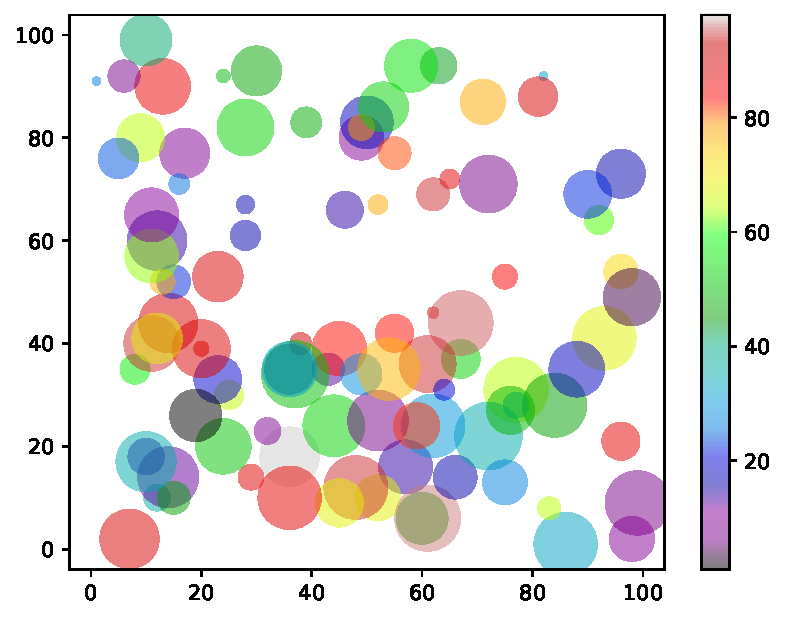
\includegraphics[scale=0.6]{img/grafica1044.pdf}
\end{figure}
\end{code}

\section{Diagrama de barras}

Con \texttt{Pyplot}, se puede utilizar la función \texttt{bar()} para dibujar gráficos de barras.\\

\begin{code} Dibuja 4 barras.

\begin{Shaded}
\begin{Highlighting}[]
\ImportTok{import}\NormalTok{ matplotlib.pyplot }\ImportTok{as}\NormalTok{ plt}
\ImportTok{import}\NormalTok{ numpy }\ImportTok{as}\NormalTok{ np}

\NormalTok{x }\OperatorTok{=}\NormalTok{ np.array([}\StringTok{"A"}\NormalTok{, }\StringTok{"B"}\NormalTok{, }\StringTok{"C"}\NormalTok{, }\StringTok{"D"}\NormalTok{])}
\NormalTok{y }\OperatorTok{=}\NormalTok{ np.array([}\DecValTok{3}\NormalTok{, }\DecValTok{8}\NormalTok{, }\DecValTok{1}\NormalTok{, }\DecValTok{10}\NormalTok{])}

\NormalTok{plt.bar(x,y)}
\NormalTok{plt.show()}
\end{Highlighting}
\end{Shaded}

\begin{figure}
  \centering
  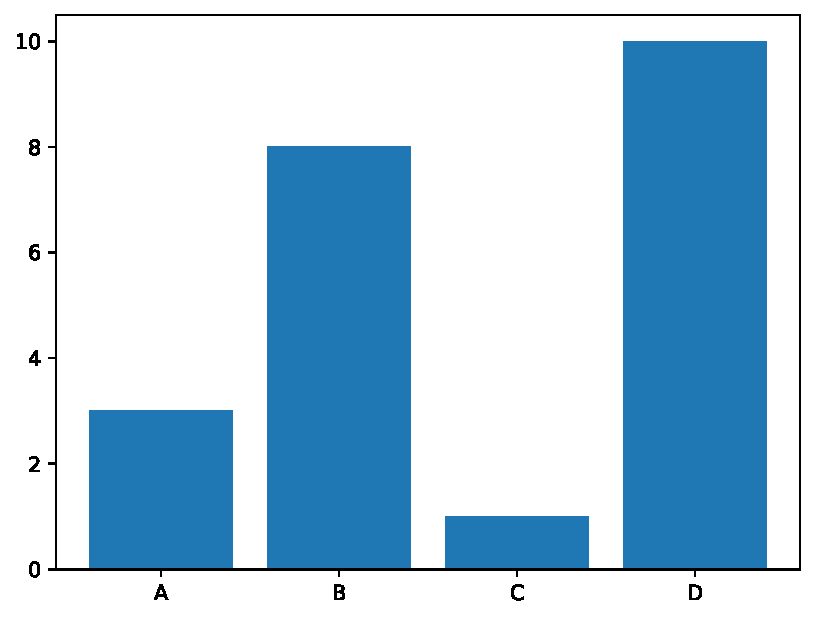
\includegraphics[scale=0.6]{img/grafica1045.pdf}
\end{figure}
\end{code}

La función \texttt{bar()} toma argumentos que describen el diseño de las
barras.

Las categorías y sus valores representados por el primer y segundo
argumento como matrices.

\section{Barras horizontales}

Si desea que las barras se muestren horizontalmente en lugar de
verticalmente, utilice la función \texttt{barh()}. \\

\begin{code} Dibuja 4 barras horizontales.

\begin{Shaded}
\begin{Highlighting}[]
\ImportTok{import}\NormalTok{ matplotlib.pyplot }\ImportTok{as}\NormalTok{ plt}
\ImportTok{import}\NormalTok{ numpy }\ImportTok{as}\NormalTok{ np}

\NormalTok{x }\OperatorTok{=}\NormalTok{ np.array([}\StringTok{"A"}\NormalTok{, }\StringTok{"B"}\NormalTok{, }\StringTok{"C"}\NormalTok{, }\StringTok{"D"}\NormalTok{])}
\NormalTok{y }\OperatorTok{=}\NormalTok{ np.array([}\DecValTok{3}\NormalTok{, }\DecValTok{8}\NormalTok{, }\DecValTok{1}\NormalTok{, }\DecValTok{10}\NormalTok{])}

\NormalTok{plt.barh(x, y)}
\NormalTok{plt.show()}
\end{Highlighting}
\end{Shaded}

\begin{figure}
  \centering
  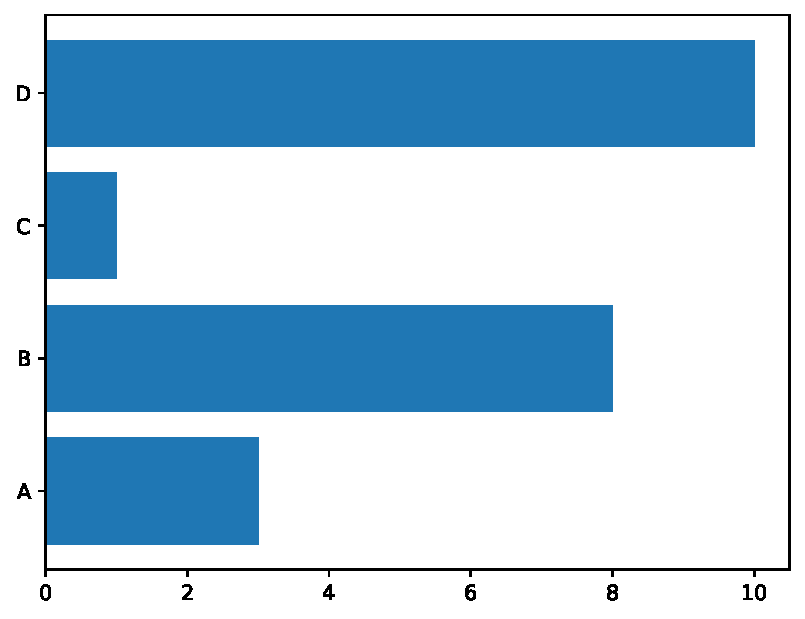
\includegraphics[scale=0.6]{img/grafica1046.pdf}
\end{figure}
\end{code}

\section{Color de la barra}

El argumento \texttt{color} de palabra clave \texttt{bar()} y
\texttt{barh()} se utiliza para establecer el color de las barras.

\begin{code} Dibuja 4 barras rojas.

\begin{Shaded}
\begin{Highlighting}[]
\ImportTok{import}\NormalTok{ matplotlib.pyplot }\ImportTok{as}\NormalTok{ plt}
\ImportTok{import}\NormalTok{ numpy }\ImportTok{as}\NormalTok{ np}

\NormalTok{x }\OperatorTok{=}\NormalTok{ np.array([}\StringTok{"A"}\NormalTok{, }\StringTok{"B"}\NormalTok{, }\StringTok{"C"}\NormalTok{, }\StringTok{"D"}\NormalTok{])}
\NormalTok{y }\OperatorTok{=}\NormalTok{ np.array([}\DecValTok{3}\NormalTok{, }\DecValTok{8}\NormalTok{, }\DecValTok{1}\NormalTok{, }\DecValTok{10}\NormalTok{])}

\NormalTok{plt.bar(x, y, color }\OperatorTok{=} \StringTok{"red"}\NormalTok{)}
\NormalTok{plt.show()}
\end{Highlighting}
\end{Shaded}

\begin{figure}
  \centering
  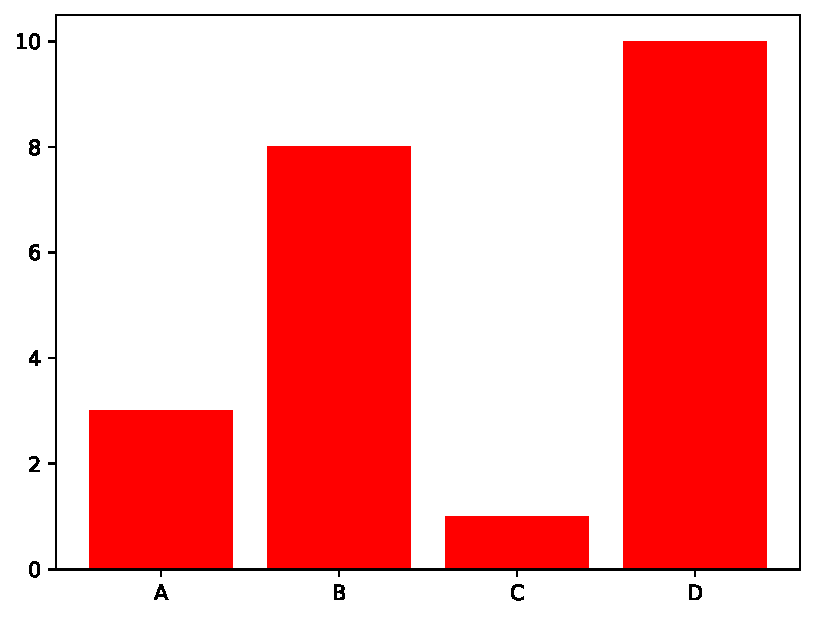
\includegraphics[scale=0.6]{img/grafica1047.pdf}
\end{figure}
\end{code}

\textbf{Nota}. Puede utilizar cualquiera de los 140 \href{https://www.w3schools.com/colors/colors_names.asp}{nombres de
colores admitidos} o valores de \href{https://www.w3schools.com/colors/colors_hexadecimal.asp}{color hexadecimales}.

\section{Ancho de barra}

El argumento \texttt{width} de palabra clave \texttt{bar()} permite
establecer el ancho de las barras. \\

\begin{code} Dibuja 4 barras muy finas.

\begin{Shaded}
\begin{Highlighting}[]
\ImportTok{import}\NormalTok{ matplotlib.pyplot }\ImportTok{as}\NormalTok{ plt}
\ImportTok{import}\NormalTok{ numpy }\ImportTok{as}\NormalTok{ np}

\NormalTok{x }\OperatorTok{=}\NormalTok{ np.array([}\StringTok{"A"}\NormalTok{, }\StringTok{"B"}\NormalTok{, }\StringTok{"C"}\NormalTok{, }\StringTok{"D"}\NormalTok{])}
\NormalTok{y }\OperatorTok{=}\NormalTok{ np.array([}\DecValTok{3}\NormalTok{, }\DecValTok{8}\NormalTok{, }\DecValTok{1}\NormalTok{, }\DecValTok{10}\NormalTok{])}
\NormalTok{width }\OperatorTok{=}\NormalTok{ np.array([}\FloatTok{0.1}\NormalTok{, }\DecValTok{1}\NormalTok{, }\FloatTok{0.5}\NormalTok{, }\FloatTok{0.7}\NormalTok{])}

\NormalTok{plt.bar(x, y, width }\OperatorTok{=}\NormalTok{ width)}
\NormalTok{plt.show()}
\end{Highlighting}
\end{Shaded}

\begin{figure}
  \centering
  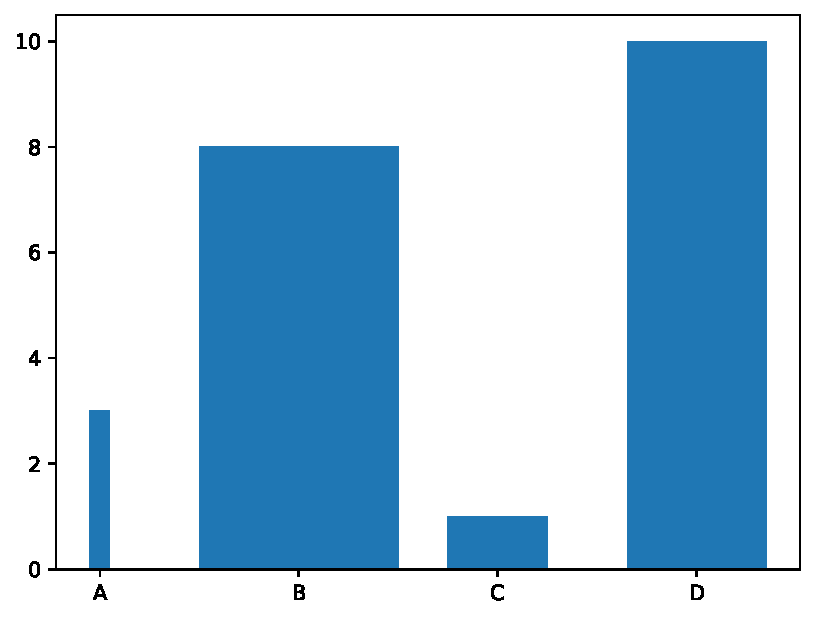
\includegraphics[scale=0.6]{img/grafica1048.pdf}
\end{figure}
\end{code}

El valor de ancho predeterminado es 0.8.

\textbf{Nota}: Para barras horizontales, utilice \texttt{height} en lugar de \texttt{width}.

\section{Histograma}

En Matplotlib, se utiliza la función \texttt{hist()} para crear histogramas.

La función \texttt{hist()} utilizará una matriz de números para crear un
histograma; la matriz se envía a la función como argumento.

A manera de ejemplo, se utiliza \texttt{NumPy} para generar una matriz
con 250 valores aleatorios, donde los valores se concentrarán alrededor
de 170 y la desviación estándar es 10. \\

\begin{code} Una distribución de datos normal por \texttt{NumPy}.

\begin{Shaded}
\begin{Highlighting}[]
\ImportTok{import}\NormalTok{ matplotlib.pyplot }\ImportTok{as}\NormalTok{ plt}
\ImportTok{import}\NormalTok{ numpy }\ImportTok{as}\NormalTok{ np}

\NormalTok{x }\OperatorTok{=}\NormalTok{ np.random.normal(}\DecValTok{170}\NormalTok{, }\DecValTok{10}\NormalTok{, }\DecValTok{250}\NormalTok{)}

\NormalTok{plt.hist(x)}
\NormalTok{plt.show() }
\end{Highlighting}
\end{Shaded}

\begin{figure}
  \centering
  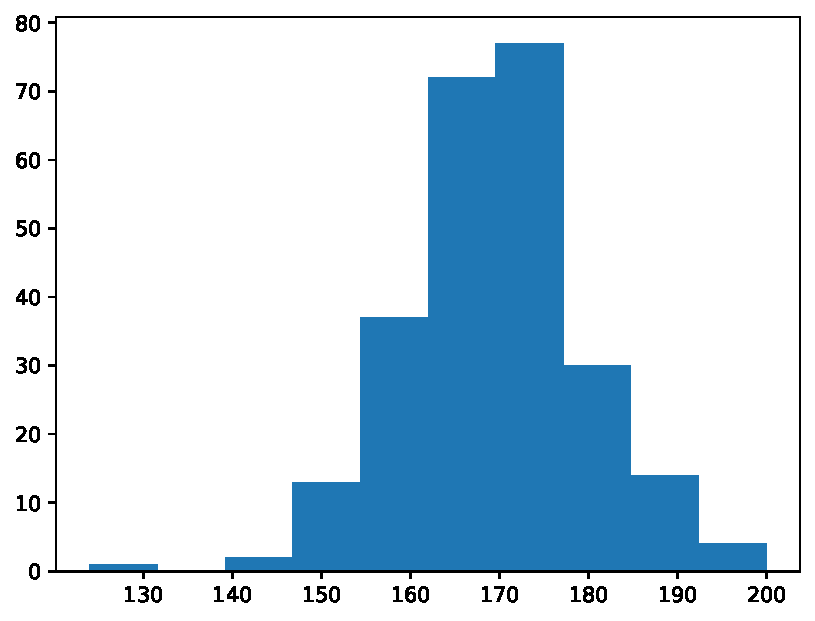
\includegraphics[scale=0.6]{img/grafica1049.pdf}
\end{figure}
\end{code}

\begin{code} Graficar las funciones Seno y Coseno.

\begin{Shaded}
\begin{Highlighting}[]
\ImportTok{import}\NormalTok{ matplotlib.pyplot }\ImportTok{as}\NormalTok{ plt}
\ImportTok{import}\NormalTok{ numpy }\ImportTok{as}\NormalTok{ np}
\ImportTok{import}\NormalTok{ matplotlib}

\NormalTok{x }\OperatorTok{=}\NormalTok{ np.linspace(}\DecValTok{0}\NormalTok{, }\DecValTok{2} \OperatorTok{*}\NormalTok{ np.pi, }\DecValTok{200}\NormalTok{)}
\NormalTok{y1 }\OperatorTok{=}\NormalTok{ np.sin(x)}
\NormalTok{y2 }\OperatorTok{=}\NormalTok{ np.cos(x)}

\NormalTok{plt.plot(x, y1, label}\OperatorTok{=}\StringTok{"Seno"}\NormalTok{)}
\NormalTok{plt.plot(x, y2, label}\OperatorTok{=}\StringTok{"Coseno"}\NormalTok{)}

\NormalTok{plt.legend()}
\NormalTok{plt.grid()}
\NormalTok{plt.title(}\StringTok{\textquotesingle{}Gráfica de las funciones Seno y Coseno\textquotesingle{}}\NormalTok{)}
\NormalTok{plt.xlabel(}\StringTok{\textquotesingle{}Ángulo en radianes\textquotesingle{}}\NormalTok{)}
\NormalTok{plt.ylabel(}\StringTok{\textquotesingle{}Valor de la función\textquotesingle{}}\NormalTok{)}

\NormalTok{plt.show()}
\end{Highlighting}
\end{Shaded}

\begin{figure}
  \centering
  \includegraphics[scale=0.6]{img/grafica1050.pdf}
\end{figure}
\end{code}

\section{Referencias}

\begin{itemize}
  \item \href{https://github.com/matplotlib/matplotlib/releases/tag/v3.9.2}{Matplotlib en GitHub}
\end{itemize}
